\synctex=1
\documentclass[11pt, a4paper]{article}

%% Packages
\usepackage{subcaption}
\usepackage{amsthm}
\usepackage{amsmath}
\usepackage{amsfonts}
\usepackage{booktabs}
\usepackage{natbib}
\usepackage{hyperref}
% \usepackage{fullpage}
\usepackage{graphicx}
\usepackage{mathtools}
\usepackage{color}
\usepackage[left = 2.5cm, right = 2.5cm, bottom = 3cm, top = 2.5cm]{geometry}
% \usepackage{enumitem}
\usepackage{multirow}
\usepackage{rotating}
\usepackage{calc}
\usepackage{bm}
\usepackage{pdfpages}
\usepackage{authblk}
\usepackage{dcolumn}
\usepackage{float}


%\usepackage[inline]{showlabels}
%\renewcommand{\showlabelfont}{\small\tt\color{red}}

%% Commands 
% \newcommand*{\bb}{}
\newcommand*{\bb}{\boldsymbol}
\newcommand{\IK}[1]{{\noindent \color{blue} \bf \#IK: #1}}
\newcommand{\PS}[1]{{\noindent \color{red} \bf \#PS: #1}}
\newcommand{\iq}[3]{#1^{#2}_{#3}}
\newcommand{\mi}[5]{\prescript{#3}{#2}{{#1}}_{#4}^{#5}}
\newcommand{\Q}[4]{\tilde Q_{#1}^{(#2,#3,#4)}}
\newcommand{\pQ}[4]{Q_{#1}^{(#2,#3,#4)}}
\newcommand{\Op}[1]{\ensuremath{{\mathcal{O}_p(#1)}}}
\newcommand{\op}[1]{\ensuremath{{o_p(#1)}}}


\newcommand{\vnorm}[1]{\ensuremath{{\left\| #1 \right\|}}}
\newcommand{\mnorm}[1]{{\left\vert\kern-0.25ex\left\vert\kern-0.25ex\left\vert #1 
		\right\vert\kern-0.25ex\right\vert\kern-0.25ex\right\vert}}
\newcommand{\mnorms}[1]{{\vert\kern-0.25ex\vert\kern-0.25ex\vert #1 
		\vert\kern-0.25ex\vert\kern-0.25ex\vert}}

       
%% Theorems etc
\newtheoremstyle{example}% name
{3pt} %Space above
{3pt} %Space below
{} %Body font
{0\parindent} %Indent amount 1
{\bf}
% {\scshape} %Theorem head font
{:} %Punctuation after theorem head
{.5em} %Space after theorem head 2
{} %Theorem head spec (
\newtheoremstyle{theorem}% name
{3pt} %Space above
{3pt} %Space below
{\em} %Body font
{0\parindent} %Indent amount 1
{\bf}
% {\scshape} %Theorem head font
{:} %Punctuation after theorem head
{.5em} %Space after theorem head 2
{} %Theorem head spec (
\theoremstyle{example} \newtheorem{example}{Example}[section]
\theoremstyle{theorem} \newtheorem{theorem}{Theorem}[section]
\newtheorem*{proposition}{Proposition}
\newtheorem{lemma}[theorem]{Lemma}


%% Definitions
\def\sign{\mathop{\rm sign}}
\def\expect{{\mathop{\rm E}}}
\def\var{{\mathop{\rm var}}}
\def\cov{{\mathop{\rm cov}}}
\def\trace{{\mathop{\rm trace}}}
\def\det{{\mathop{\rm det}}}

\def\bbeta{\bb{\beta}}
\def\btheta{\bb{\theta}}
\def\bgamma{\bb{\gamma}}
\def\bSigma{\bb{\Sigma}}
\def\bgamma{\bb{\gamma}}
\def\by{\bb{y}}
\def\bC{\bb{C}}
\def\bY{\bb{Y}}
\def\bu{\bb{u}}
\def\bx{\bb{x}}
\def\bz{\bb{z}}
\def\b0{\bb{0}}
\def\bX{\bb{X}}
\def\bZ{\bb{Z}}
\def\bv{\bb{v}}
\def\bV{\bb{V}}
\def\bY{\bb{Y}}
\def\by{\bb{y}}
\def\bL{\bb{L}}
\def\bLt{\tilde{\bb{L}}}
\def\btnod{\bb{\theta}_0}
\def\bttilde{\tilde{\bb{\theta}}}
\def\bW {\bb{W}}
%% Title Page 
\title{Maximum softly-penalized likelihood for Bernoulli-response generalized linear mixed models}
 
\author[1]{Philipp Sterzinger}
\author[1,2]{Ioannis Kosmidis}

\affil[1]{Department of Statistics, University of Warwick, Coventry, CV4 7AL, UK}
\affil[2]{The Alan Turing Institute, London, NW1 2DB, UK}


\begin{document}
\maketitle
%\tableofcontents

\begin{abstract}
  We introduce a soft penalization approach for stabilizing maximum
  likelihood estimation in Bernoulli-response generalized linear mixed
  models, which is known to have a positive probability to result in
  estimates on the boundary of the parameter space. Such estimates, instances of which
  are infinite values for fixed effects and singular or
  infinite variance components, can cause havoc to numerical
  estimation procedures and inference. We introduce an additive penalty to the log-likelihood function, 
  which consists of appropriately scaled versions of the Jeffreys
  prior for the model with no random effects and the negative Huber loss. The resulting maximum softly-penalized likelihood
  estimates are shown to lie in the interior of the parameter
  space. Appropriate scaling of the penalty guarantees that the penalization is soft-enough to recover
  the optimal asymptotic properties expected by the maximum likelihood
  estimator, namely consistency, asymptotic normality,
  Cram\'{e}r-Rao efficiency and asymptotically valid hypothesis testing. Further, our choice of penalties and scaling factor preserves invariance of the fixed effects estimates under linear transformation of the model
  parameters, such as contrasts. Maximum softly-penalized likelihood
  is compared to competing approaches on two real-data examples,
  and comprehensive simulation studies that illustrate its superior finite sample
  performance.
  \bigskip \\
  \noindent {Keywords: logistic regression, infinite estimates, singular variance components, data separation, Jeffreys prior}
\end{abstract}

\section{Introduction}
\label{sec:intro}

Generalized Linear Mixed Models (GLMMs; \citealt[Chapter
7]{mcculloch+etal:2008}) are a potent class of statistical models
that allow associating Gaussian and non-Gaussian responses, such as
counts, proportions, positive responses, and so on, with covariates,
while accounting for complex multivariate dependencies. This is achieved by linking
the expectation of a response to a linear combination of covariates
and parameters (fixed effects), and sources of extra variation (random
effects) with known distributions. Although these models find
application in numerous fields such as biology, ecology and the social
sciences \citep{bolker+etal:2009}, estimation of GLMMs is not
straightforward in practice, because their likelihood is generally an intractable
multivariate integral.

Maximum approximate likelihood (MAL) methods maximize an 
approximation of the GLMM likelihood, that can, in principle, be
chosen to be arbitrarily accurate \citep[see, for example,
][]{raudenbush+etal:2000, pinheiro+chao:2006}. Such methods are
pervasive in contemporary GLMM practice because, like maximum
likelihood (ML), MAL estimators are consistent under general conditions
about the model, and the MAL estimates and the approximate likelihood
itself can be used for the construction of likelihood-based
inferences, such as likelihood-ratio tests or Wald
statistics, and can be used for model selection based on information criteria. An
alternative approach to MAL are Bayesian posterior update procedures
\citep[see, for example,][]{zhao+etal:2006,browne+draper:2006}. However, they come with
various technical difficulties, such as determining the scaling of the
covariates, selecting appropriate priors, coming up with efficient
posterior sampling algorithms, and determining burn-in times of chains
for reliable estimation. Yet another alternative to MAL are maximum
penalized quasi-likelihood (MPQL) methods \citep{schall:1991,
  wolfinger+oconnel:1993, breslow+clayton:1993} which essentially fit a Linear Mixed Model to transformed pseudo-responses. However, the penalized quasi likelihood may not
yield an accurate approximation of the GLMM likelihood. As a result,
MPQL estimators can have large bias when the random effects
variances are large
\citep{bolker+etal:2009,rodriguez+goldman1995} and are
not necessarily consistent \citep[Chapter 3.1]{jiang:2017}.

Despite the pervasiveness of MAL, certain data configurations can
result in MAL estimates of the variance-covariance matrix of the
random effects distribution to be on the boundary of the parameter
space, such as infinite or zero estimated variances, or, more
generally, singular estimates of the variance-covariance matrix; see
\cite{chung+etal:2013} for an excellent discussion. In
addition, as is the case in maximum likelihood estimation of
Bernoulli-response generalized linear models \citep[GLMs; see, for
example][Chapter 4]{mccullagh+nelder:1989}, the MAL estimates of the
fixed effects can be
infinite. As is well-acknowledged in the GLMM literature \citep[see,
for example][]{bolker+etal:2009, bolker:2018,
  pasch+etal:2013}, both instances of boundary estimates can
cause havoc to numerical optimization procedures used for MAL. In
addition, if they go undetected, they can substantially impact
first-order inferential procedures, like Wald tests, resulting in
spuriously strong or weak conclusions. In contrast to the
numerous approaches to detect (see, for example,
\citealt{kosmidis+schumacher:2021} for the \texttt{detectseparation} R
package that implements the methods in \citealt{konis:2017}) and
handle \citep[see, for example,][]{kosmidis+firth:2020,
 heinze+schemper:2002, gelman+etal:2008} infinite
estimates in Bernoulli-response GLMs, little methodology or guidance
is available on how to detect or deal with degenerate estimates in
GLMMs.

We introduce a maximum softly-penalized approximate likelihood (MSPAL)
procedure for Bernoulli-response GLMMs that returns estimators that
are guaranteed to take values in the interior of the parameter space,
and are also consistent, asymptotically normal, Cram\'{e}r-Rao
efficient and give asymptotically valid inference, under no additional assumptions beyond those typically
required for establishing consistency, asymptotic normality, and asymptotically valid inference of MAL
or ML estimators. Although the developments here are for
Bernoulli-response GLMMs, they provide a blueprint for the
construction of penalties and estimators with values in the interior
of the parameter space for any GLMM and, more generally, for
M-estimation settings where boundary estimates occur. The
(approximate) likelihood penalty we introduce consists of
appropriately scaled versions of the Jeffreys prior for the model with
no random effects, and the negative Huber loss. We show that the MSPAL
estimates are guaranteed to be in the interior of the parameter space,
and impose a scaling to the penalty
that guarantees that i) penalization is soft-enough for the MSPAL
estimator to have the optimal asymptotic properties expected by the ML
estimator, and ii) that the fixed effects estimates are invariant to linear
transformation of the model parameters, such as contrasts, in the
sense that the MSPAL estimates of linear transformations of the fixed
effects parameters are the linear transformations of the MSPAL
estimates. Both i) and ii) are in contrast to other penalization
procedures that have been proposed in the literature \citep[see, for
example,][]{chung+etal:2013, chung+etal:2015}. Maximum
softly-penalized likelihood is compared to prominent competing
approaches through two real-data examples, and comprehensive
simulation studies that illustrate its superior finite-sample
performance. 

The remainder of the paper is organized as follows. Section \ref{sec:bern_GLMMs} defines the clustered
Bernoulli-response GLMM and Section \ref{sec:culcita_dat} gives a motivating real-data example of
degenerate maximum approximate likelihood estimates in a Bernoulli-response GLMM. Section
\ref{sec:softpen} formalizes the maximum softly penalized approximate likelihood framework and
states the large sample results of the softly penalized maximum
likelihood estimator. Section \ref{sec:ci} demonstrates the performance of the MSPAL on another real-data example and a data-based simulation and Section \ref{sec:sum} provides concluding remarks. Proofs, details on the simulations in this paper and further simulations on synthetic data are given in the supplementary material. 

\section{Bernoulli-response generalized linear mixed models}
\label{sec:bern_GLMMs}

Suppose that response vectors $\by_1, \ldots, \by_k$ are observed with
$\by_i = (y_{i1}, \ldots, y_{in_i})^\top \in \{0, 1\}^{n_i}$, possibly
along with covariate matrices $\bV_1, \ldots, \bV_k$, respectively,
where $\bV_i$ is a $n_i \times s$ matrix.

A Bernoulli-response GLMM assumes that $\by_1, \ldots, \by_k$
are realizations of random vectors $\bY_1, \ldots, \bY_k$, whose entries
$Y_{i1}, \ldots, Y_{in_i}$ $(i = 1, \ldots, k)$ are independent
Bernoulli random variables conditionally on a vector of random effects
$\bu_i$. The vectors $\bu_1, \ldots, \bu_k$ are assumed to be
independent realizations of a multivariate normal distribution, and the conditional mean of each Bernoulli random
variable is linked to a linear predictor $\eta_{ij}$, which is a
linear combination of covariates with random effects and fixed effects.
Specifically,
\begin{align}
\label{eq:bern_cluster}
  Y_{ij} \mid \bb{u}_i & \sim \text{Bernoulli}(\mu_{ij}) \quad \text{with} \quad
  g(\mu_{ij}) = \eta_{ij} = \bx_{ij}^\top \bbeta + \bz_{ij}^\top \bu_i\\
  \bu_i & \sim \text{N}(\b0_q, \bb{\Sigma})  \quad (i = 1, \ldots, k; j = 1, \ldots, n_i)\,,
\end{align}
where $\mu_{ij} = P(Y_{ij} = 1 \mid \bu_i, \bx_{ij}, \bz_{ij})$, and
$g: (0, 1) \to \Re$ is a known monotone increasing link function, like
the logistic, probit or complementary log-log. The vector $\bx_{ij}$
is the $j$th row of the $n_i \times p$ model matrix $\bX_{i}$
associated with the $p$-vector of fixed effects
$\bbeta \in \Re^p$, and $\bz_{ij}$ is the $j$th row of the
$n_i \times q$ model matrix $\bZ_{i}$ associated with the $q$-vector
of random effects $\bu_i$. The model matrices $\bX_i$ and $\bZ_i$ are
formed from subsets of columns of $\bV_i$. The variance-covariance
matrix $\bSigma$ collects the variance components and is assumed to be
symmetric and positive definite. The Bernoulli-response GLMM
in~(\ref{eq:bern_cluster}) is here introduced explicitly in terms of
clusters. The other often encountered formulation of GLMMs in the literature \citep[Chapter 7.4]{mcculloch+etal:2008} absorbs the clustering into the variance components structure of $\bSigma$ and is therefore a clustered GLMM with a single cluster. Hence, the presentation and results here are with no loss
of generality.

The marginal likelihood about $\bb{\beta}$ and $\bb{\Sigma}$ for
model~(\ref{eq:bern_cluster}) is
\begin{equation}
\label{eq:bern_likl}
L(\bbeta,\bSigma) = (2\pi)^{-kq/2} \det(\bSigma)^{-k/2} \prod_{i=1}^{k}\int_{\Re^q}\prod_{j=1}^{n_i} \mu_{ij}^{y_{ij}}(1-\mu_{ij})^{1-y_{ij}} \exp\left\{-\frac{\bu_i^\top\bSigma^{-1}\bu_i}{2} \right\} d\bu_i\,,
\end{equation}
Formally, the ML estimator is the maximizer of~(\ref{eq:bern_likl})
with respect to $\bbeta$ and $\bSigma$. However,
(\ref{eq:bern_likl}) involves intractable integrals, which are
typically approximated before maximization, resulting in MAL
estimators. For example, the popular \texttt{glmer} routine of the
R \citep{R} package \texttt{lme4} \citep{bates+etal:2015} uses adaptive
Gauss-Hermite quadrature for one-dimensional random effects and
Laplace approximation for higher-dimensional random effects. A
detailed account of those approximation methods can be found in
\citet{pinheiro+bates:1995}.
% The custom implementations of~(\ref{eq:bern_likl}) in the current work
% use Gauss-Hermite quadrature approximations of~(\ref{eq:bern_likl})
% for one-dimensional random effects models, and a Laplace approximation
% of~(\ref{eq:bern_likl}) for higher dimensions

\section{Motivating example}
\label{sec:culcita_dat}

The working data set in this section is a reduced version of the data
in \citet{mckeon+etal:2012}, as provided in the worked examples of
\citet{bolker:2015} (available at
\url{https://bbolker.github.io/mixedmodels-misc/ecostats\_chap.html}). The
data is given in Table~\ref{tab:culcita} and comes from trials
involving coral-eating sea stars Culcita novauguineae (hereafter
Culcita) attacking coral that harbour differing combinations of
protective symbionts, involving crabs and shrimp. The design is a
randomised complete block design with two replications per treatment
per block, four treatments, involving no symbionts, crabs only, shrimp
only, both crabs and shrimp, and ten temporal blocks. As a result
there is a total of 80 observations on whether predation was present
(recorded as one) or not (recorded as zero). By mere inspection
of Table~\ref{tab:culcita}, we note that predation becomes more prevalent
with increasing block number, and that predation gets suppressed when either
crabs or shrimp are present, and more so when both symbionts are
present. The only observation that deviates from this general trend is the observation in block 10 with no predation and no symbionts.

  \begin{table}[t]
    \caption{Culcita data \citep{mckeon+etal:2012} from the worked
      examples of \citet{bolker:2015} (available at
      \url{https://bbolker.github.io/mixedmodels-misc/ecostats\_chap.html}).}
    \label{tab:culcita}
    \centering
    \begin{tabular}{lllllllllll}
      \toprule
      & \multicolumn{10}{c}{Block} \\ \cmidrule{2-11}
      \multicolumn{1}{c}{Treatment} & \multicolumn{1}{c}{1} & \multicolumn{1}{c}{2} & \multicolumn{1}{c}{3} & \multicolumn{1}{c}{4} & \multicolumn{1}{c}{5} & \multicolumn{1}{c}{6} & \multicolumn{1}{c}{7} & \multicolumn{1}{c}{8} & \multicolumn{1}{c}{9} & \multicolumn{1}{c}{10} \\
      \midrule
      none & 0,1 & 1,1 & 1,1 & 1,1 & 1,1 & 1,1 & 1,1 & 1,1 & 1,1 & 1,0 \\
      crabs & 0,0 & 0,0 & 0,0 & 0,0 & 1,1 & 1,1 & 1,1 & 1,1 & 1,1 & 1,1 \\
      shrimp & 0,0 & 0,0 & 0,0 & 0,0 & 0,1 & 1,1 & 1,1 & 1,1 & 1,1 & 1,1 \\
      both & 0,0 & 0,0 & 0,0 & 0,0 & 0,0 & 0,1 & 1,1 & 1,1 & 1,1 & 1,1 \\
      \bottomrule
    \end{tabular}
\end{table}

A Bernoulli-response GLMM with one random intercept per block can be
used here to associate predation to treatment effects while
accounting for heterogeneity between blocks. Such a model can be
defined as
\begin{align}
  \label{eq:logistic_normal}
  Y_{ij} \mid u_i & \sim \text{Bernoulli}(\mu_{ij}) \quad  \text{with} \quad
  \log{\frac{\mu_{ij}}{1 - \mu_{ij}}} =  \eta_{ij} =  \beta_0 + u_i + \beta_{j} \\ 
  u_i & \sim \text{N}(0, \sigma^2) \quad (i = 1, \ldots, 10; j = 1, \ldots, 4)\,.
\end{align}
In the above expressions, $Y_{i1}$, $Y_{i2}$, $Y_{i3}$, and $Y_{i4}$
correspond to responses for ``none'', ``crabs'', ``shrimp'', ``both'',
respectively, and we set $\beta_1 = 0$ for identifiability purposes,
effectively using ``none'' as a reference category. The logarithm of the model likelihood~(\ref{eq:bern_likl}) about the parameters
$\bbeta = (\beta_0, \beta_2, \beta_3, \beta_4)^\top$ and
$\psi = \log\sigma$ for model~(\ref{eq:logistic_normal}) is
approximated using an adaptive quadrature rule with $Q = 100$ points
\citep[see, for example,][]{liu+pierce:1994, pinheiro+bates:1995} as
implemented in \texttt{glmer}.  The approximation to the log-likelihood
gets more accurate as the number of quadrature points increases, and
here we choose $Q = 100$ points, which is the maximum possible in the
current \texttt{glmer} implementation.

All parameter estimates of model~(\ref{eq:logistic_normal})
reported in the current example are computed after removing the
atypical observation with zero predation in block 10 when there are no
symbionts. Estimates based on all data points are provided in
Table~\ref{XXX} of the supplementary materials \IK{include that}.

The MAL estimates of $\bbeta$ and $\psi$ in
Table~\ref{tab:culcita_inf} are computed using the numerical
optimization procedures ``BFGS'' and ``CG'' (MAL(BFGS) and MAL(CG),
respectively), as these are readily available from the \texttt{optimx} R
package \citep[see][Section 3 for details]{nash+varadhan:2011}, with
default starting values. The MAL(BFGS) and MAL(CG) estimates are different,
and are notably extreme on the logistic scale. This is due to the two
optimization procedures stopping early at different points in the
parameter space after having prematurely declared convergence. The large estimated
standard errors are indicative of the approximation
to the log-likelihood being almost flat around the estimates. In this
case, the MAL estimates for the fixed effects
$\beta_0, \beta_1, \beta_2, \beta_3$ are in reality infinite in
absolute value.

\begin{table}[t]
  \caption{Estimates from the degenerate Culcita subdataset of \citet{bolker:2015} using MAL,MSPAL and \texttt{bglmer} } 
  \label{tab:culcita_inf}
  \centering
  \begin{tabular}{lD{.}{.}{3}D{.}{.}{3}D{.}{.}{3}D{.}{.}{3}D{.}{.}{3}}
    \toprule
%     &
% \multicolumn{2}{c}{MAL} &
% \multicolumn{2}{c}{bglmer} & 
% \multicolumn{1}{c}{MSPAL} \\ \cmidrule{2-3}\cmidrule{4-5}
&
\multicolumn{1}{c}{MAL(BFGS)} & 
\multicolumn{1}{c}{MAL(CG)} &
\multicolumn{1}{c}{bglmer(t)} &
\multicolumn{1}{c}{bglmer(n)} & \multicolumn{1}{c}{MSPAL}
    \\
\midrule
\multicolumn{6}{c}{reference category: ``none''} \\
\midrule
$\beta_0$ & 15.88 & 15.37 & 6.39 & 4.90 & 8.41\\
            & (10.14) & (9.50) & (2.60) & (2.08) & (3.43)\\
$\beta_2$    & -12.93 & -12.46 & -4.02 & -2.84 & -7.22\\
            & (9.15) & (8.53) & (1.59) & (1.27) & (3.21)\\
$\beta_3$   & -14.81 & -14.30 & -4.81 & -3.44 & -8.26\\
            & (9.89) & (9.24) & (1.73) & (1.35) & (3.48)\\
$\beta_4$     & -17.71 & -17.15 & -6.47 & -4.73 & -10.10\\
            & (10.70) & (10.02) & (2.05) & (1.57) & (3.84)\\
$\log\sigma$   & 2.31 & 2.28 & 1.72 & 1.54 & 1.80\\
            & (0.64) & (0.62) & (0.44) & (0.43) & (0.45)\\
\midrule
\multicolumn{6}{c}{reference category: ``both''} \\
\midrule
$\gamma_0$ & -1.82 & -1.74 & 0.37 & 0.57 & -1.70\\
            & (3.92) & (3.77) & (2.24) & (2.07) & (2.46)\\
$\gamma_1$    & 17.74 & 17.09 & 6.70 & 5.75 & 10.10\\
            & (10.75) & (10.03) & (2.19) & (1.88) & (3.84)\\
$\gamma_2$   & 4.78 & 4.65 & 1.63 & 1.26 & 2.88\\
            & (3.08) & (2.98) & (1.43) & (1.32) & (1.85)\\
$\gamma_3$   & 2.89 & 2.83 & 0.83 & 0.56 & 1.85\\
            & (2.27) & (2.22) & (1.35) & (1.28) & (1.60)\\
$\log\sigma$   & 2.31 & 2.28 & 1.74 & 1.66 & 1.80\\
            & (0.64) & (0.62) & (0.44) & (0.44) & (0.45)\\
\bottomrule
  \end{tabular}
\end{table}


Parameter estimates are also obtained using the \texttt{bglmer}
routine of the \texttt{blme} R package \citep{chung+etal:2013} that has
been developed to ensure that parameter estimates from GLMMs are away
from the boundary of the parameter space. The estimates shown in
Table~\ref{tab:culcita_inf} are obtained using a penalty for $\sigma$
inspired by a gamma prior (default in \texttt{bglmer}; see
\citealt{chung+etal:2013} for details) and two of the default prior
specifications for the fixed effects: i) independent normal priors
(``bglmer(n)''), and ii) independent t priors (``bglmer(t)''), as
these are implemented in \texttt{blme}; see \texttt{bmerDist-class} in
the help pages of \texttt{blme} for details. We also show the
estimates obtained using the MSPAL estimation method that we propose
in the current work.

The maximum penalized approximate likelihood estimates from
\texttt{bglmer} and the corresponding estimated standard errors appear to
be finite. Nevertheless, the use of the default priors directly breaks
parametrization invariance under contrasts, which MAL estimates
enjoy. For example, Table~\ref{tab:culcita_inf} also shows the
estimates of model~(\ref{eq:logistic_normal}) with
$\eta_{ij} = \gamma_0 + u_i + \gamma_{j}$, where $\gamma_{4} = 0$,
i.e.~setting ``both'' as a reference category. Hence, the identities
$\gamma_0 = \beta_0 + \beta_4$, $\gamma_1 = -\beta_4$,
$\gamma_2 = \beta_2 - \beta_4$, $\gamma_3 = \beta_3 - \beta_4$ hold,
and it is natural to expect those identities from the estimates of
$\bbeta$ and $\bgamma$. As is evident from
Table~\ref{tab:culcita_inf}, the \texttt{bglmer} estimates with either
normal or t priors can deviate substantially from those
identities. For example, the \texttt{bglmer} estimate of $\gamma_1$
based on normal priors is $5.75$ while that for $\beta_4$ is $-4.73$,
and the estimate of $\log\sigma$ is $1.54$ in the $\bbeta$
parametrization and $1.66$ in the $\bgamma$
parametrization. Furthermore, different contrasts give varying
amounts of deviations from these identities. On the other hand, the
approximate likelihood is invariant to monotone parameter
transformations. As a result, the corresponding identities hold
exactly for the MAL estimates with the deviations observed in
Table~\ref{tab:culcita_inf} being due to early stopping of the optimization routines.

The \texttt{bglmer} estimates are typically closer to zero in absolute
value than the MAL estimates because the normal and t priors are all
centred at zero. Furthermore, the estimates using normal priors tend
to shrink more towards zero than those using t priors, because the
latter have heavier tails than the former. In order to assess the
impact of shrinkage on the frequentist properties of the estimators,
we simulate $10000$ independent samples of responses for the randomized
complete block design in Table~\ref{tab:culcita}, at the MAL estimates
in the $\bbeta$ parametrization when all data points are used (see
Table~\ref{XXX} of the Supplementary Materials  \IK{include that}). For each sample, we
compute the MAL and MSPAL estimates, as well as the \texttt{bglmer} estimates based on
normal and t priors.

\begin{figure}[t]
  \begin{center}
    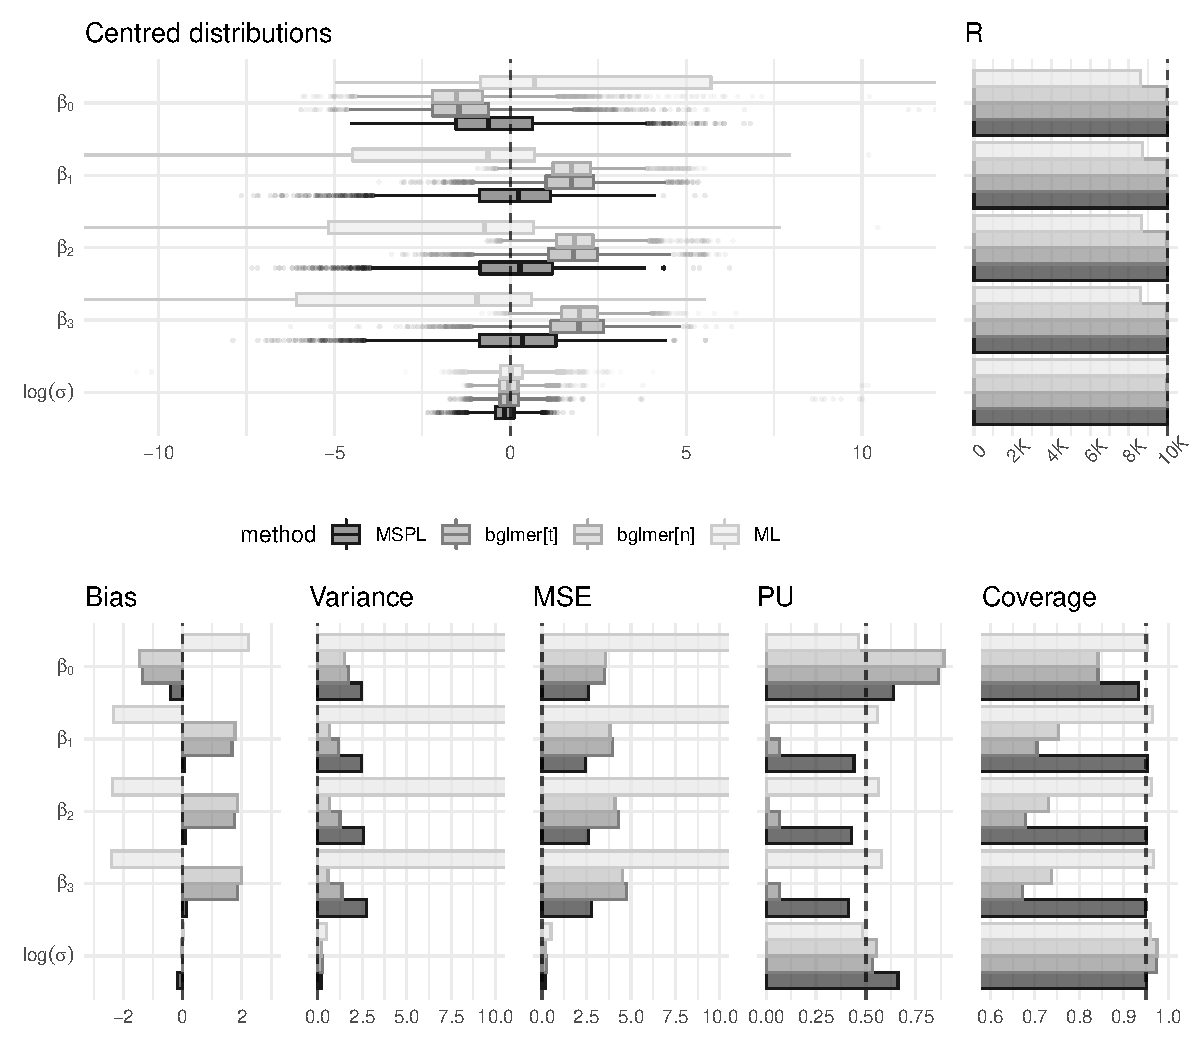
\includegraphics[width = \textwidth]{Figures/simulation_results.pdf}
  \end{center}
  \caption{Performance metrics for parameter estimates of MAL,MSPAL and \texttt{bglmer} from simulating a Bernoulli-response GLMM from the Culcita data at the MAL}
  \label{fig:culcita_simu0}
\end{figure}

Figure~\ref{fig:culcita_simu0} shows boxplots for the sampling
distributions of the estimators, centred at the true value, the estimated
finite-sample bias, variance, mean squared error, and probability of
underestimation for each estimator, along with the estimated coverage
of 95\% Wald confidence intervals based on the estimates and estimated
standard errors from the negative Hessian of the approximate
log-likelihood at the estimates. The plotting range for the support of
the distributions has been restricted to $(-11, 11)$, which does not
contain all MAL estimates in the simulation study but contains all
estimates for the other methods. We should note here that apart from
the estimated probability of underestimation,
estimates for the other summaries are not well-defined for MAL,
because the probability of boundary estimates is positive. In fact,
there were issues with at least one of the MAL estimates for $9.25\%$
of the simulated samples. These issues are either due to convergence
failures or because the estimates or estimated standard errors have
been found to be atypically large in absolute value. The displayed
summaries for MAL are computed based only on estimates which have not
been found to be problematic. Clearly, the amount of shrinkage induced
by the normal and t priors is excessive. Although the resulting
estimators have small finite-sample variance (with the one based on
normal priors having the smallest), they have excessive finite-sample
bias, which is often at the order of the standard deviation resulting
in large mean squared errors, and the sampling distributions to be
located far from the respective true values. Importantly, the
combination of small variance and large bias readily impacts
first-order inferences; Wald-type confidence intervals about the fixed
effects are found to systematically undercover the true parameter
value. Finally, both bglmer(n) and bglmer(t) do not appear prevent extreme positive variance estimates.

As is apparent from Table~\ref{tab:culcita_inf}, the identities on the
model parameters hold exactly with the proposed MSPAL estimates, where the observed deviations are attributed to rounding errors. Furthermore, from
Figure~\ref{fig:culcita_simu0} we see that the penalty we propose not only ensures
that estimates are away from the boundary of the parameter space, but
its soft nature guarantees that estimators have the optimal
frequentist properties that would be expected by the MAL estimator
had it not taken boundary values. 


\section{Penalized likelihoods}
\label{sec:softpen}

\subsection{Setup}

Suppose that we observe the values $\by_1, \ldots, \by_k$ of a
sequence of random vectors $\bY_1, \ldots, \bY_k$ with
$\by_i = (y_{i1}, \ldots, y_{in_i})^\top \in \mathcal{Y} \subset
\Re^{n_i}$, possibly with a sequence of covariate vectors
$\bv_1, \ldots, \bv_k$, with
$\bv_i = (v_{i1}, \ldots, v_{is})^\top \in \mathcal{X} \subset
\Re^{s}$. Let $\bY = (\bY_1^\top, \ldots, \bY_k^\top)^\top$, and
denote by $\bV$ the set of $\bv_1, \ldots, \bv_k$. Further, assume that the data generating process of $\bY$, conditional on $\bV$ has a density or
probability mass function $f(\bY \mid \bV; \btheta)$, indexed by a
parameter $\btheta \in \Theta \subset \Re^d$. Denote the parameter that identifies the conditional distribution of $\bY$ given $\bV$ by $\btnod \in \Theta$. 

A popular method for estimating the parameter vector $\btnod$ is to
maximize the logarithm of the likelihood $f(\bY \mid \bV; \btheta)$ with respect to
$\btheta$. If the likelihood is not
available in closed form then an approximation of it may be maximized
instead. For example, expression~(\ref{eq:bern_likl}) gives
$f(\bY \mid \bV; \btheta)$ in the case of the Bernoulli-response GLMMs
of Section~\ref{sec:bern_GLMMs}, and in Section~\ref{sec:culcita_dat}
we use an adaptive Gauss-Hermite quadrature approximation to the
log-likelihood. In what follows, $\ell(\btheta)$ denotes either the
log-likelihood or an approximation to it whenever that distinction is
immaterial for the context. Furthermore, the dependence of
$\ell(\btheta)$ on $\bY$ and $\bV$ is suppressed for notational
convenience. Then, the ML (or MAL) estimator of $\btheta$ is defined
as $\hat\btheta = \arg \max_{\btheta\in \Theta} \ell(\btheta)$.

Let $\tilde\btheta$ be the the maximum penalized likelihood (MPL) (or
maximum penalized approximate likelihood; MPAL) estimator
\[
  \tilde\btheta = \arg\max_{\btheta \in \Theta} \{\ell(\btheta) + P(\btheta) \} \, ,
\]
where $P(\btheta)$ is an additive penalty to $\ell(\btheta)$ that may depend on $\bY$ and $\bV$. 

In the remainder of this section we derive the conditions that
$P(\btheta)$ must satisfy to ensure that the MPL or MPAL
estimator $\tilde\btheta$ i) takes values always in the interior of
$\Theta$, ii) is invariant under linear transformations of the
parameters, such as scaled contrasts that are usually employed with
categorical covariates in regression modelling, and iii) has similar first order asymptotics to $\hat{\btheta}$. We then derive a penalty that satisfies
those conditions for Bernoulli-response GLMMs.

\subsection{Interior point parameter estimates}
\label{sec:interior}
Denote by $\partial \Theta$ the boundary of the parameter space, and
let $\btheta(r)$, $r \in \Re$, be a path in the parameter space such
that $\lim_{r \to \infty}\btheta(r) \in \partial \Theta$. A common
approach to resolving issues with ML or MAL estimates being in
$\partial \Theta$, like those encountered in the example of
Section~\ref{sec:culcita_dat}, is to instead use MPL or MPAL
estimators from a penalty that satisfies
$\lim_{r \to \infty} P(\btheta(r)) = -\infty$ and which are bounded from above. Then, if there is at
least one point $\btheta \in \Theta$ such that
$\ell(\btheta)  > -\infty$, it must hold that
$\tilde\btheta$ is in the interior of $\Theta$.

For example, the penalties arising from the independent normal and
independent t prior structures implemented in \texttt{blme} are such
that $\lim_{r \to \infty} P(\btheta(r)) = -\infty$, whenever
$\btheta(r)$ diverges to the boundary of the parameter space for the
fixed effects. As a result, the bglmer(n) and bglmer(t) estimates for
the fixed effects in Table~\ref{tab:culcita_inf}) are finite. On the
other hand, the default gamma-prior like penalty used in
\texttt{bglmer} for the variance component $\sigma$ is
$-1.5 \log\sigma$, which, while it ensures that the estimate of
$\log \sigma$ is not minus infinity, does not guard from positive
infinite estimates. This is apparent in
Figure~\ref{fig:culcita_simu0}, where several extreme positive
bglmer(n) and bglmer(t) estimates are observed for $\log\sigma$; see,
also, the vignettes of the \texttt{glmmsr} \citep{ogden:2019} R package
for an example with infinite variance component estimate in a
Bernoulli-response GLMM.

\subsection{Invariance under scaled linear transformations}

The ML estimates are known to be invariant to transformations of the
model parameters \citep[see, for example][]{zehna:1966}. A
particularly useful class of transformations in regression modelling
with categorical covariates is the collection of scaled linear transformations
$\btheta' = \bC \btheta$ for known, invertible, real matrices
$\bC$. With such transformations one can obtain ML or MAL estimates and corresponding
estimated standard errors for arbitrary sets of scaled parameter
contrasts, when estimates for one of those sets of contrasts are
available and with no need to re-estimate the model. Further, these transformations eliminate estimation and
inferential ambiguity when two independent researchers analyse the
same data set using the same model but with different contrasts,
e.g. due to software defaults.

The example in Section~\ref{sec:culcita_dat} shows that not all MPL or
MPAL estimators are invariant to linear transformations of the
parameters. The condition required for achieving invariance is that
the penalty satisfies $P(\bC\btheta) = P(\btheta) + b$, where
$b \in \Re$ is a real constant. This requirement does not hold for
the penalties arising from the normal and t prior structures that are
used to compute the bglmer(n) and bglmer(t) fixed effect estimates in Table~\ref{tab:culcita_inf}. Hence, the bglmer(n) and
bglmer(t) MPAL estimates are not invariant under linear
transformations of the parameters.

\subsection{Asymptotic properties}
\label{sec:ass+res}

Consistency, asymptotic normality and valid asymptotic hypothesis testing of the proposed MSPAL estimator follow readily from similar such results for MAL estimators where the approximation error to the model log-likelihood is an additive error term. Indeed, the results presented in this section are a direct translation of the work of \citet{ogden:2017}, where the term ``approximation error'' is replaced by ``penalty function''. To state the results and their underlying assumptions, we introduce some further notation. Proofs are given in Section S2 of the supplementary material.

Let $S(\btheta) $ be the score function of $\ell(\btheta)$, i.e. $S(\btheta ) =\nabla \ell(\btheta)$, and let $\tilde{S}(\btheta) = \nabla\ell(\btheta) + \nabla P(\btheta)$ be the score of its penalized analogue $\tilde{\ell}(\btheta) = \ell(\btheta)+P(\btheta)$. Denote the observed information matrix by $J(\btheta) = -\nabla \nabla^\top \ell(\btheta)$. It is assumed that information regarding the model parameter accumulates at a rate $r_n$ in the sense that $r_n^{-1}J(\btheta ) \overset{p}{\to} I(\btheta)$ as $n \to \infty$ for some nonrandom, positive definite, $\mathcal{O}(1)$, matrix $I(\btheta)$ and with respect to some matrix norm $\mnorm{\cdot}$. Further, let $\delta(\btheta) = \vnorm{\nabla P(\btheta)}$ % and $\gamma(\theta)=\norm{ J(\theta)-\tilde{J}(\theta)}$ 
for some vector norm $\vnorm{\cdot}$, and for $S \subseteq \Theta$ define $\delta^\infty(S)  = \underset{\btheta \in S}{\sup} \; \delta(\btheta)$ and $\delta^\infty = \delta^\infty(\Theta)$. Finally, denote by $B_t(\btheta)$ the ball of radius $t$ around $\btheta$. 

We impose standard M-estimation regularity conditions on the score function to establish consistency of $\bttilde$ (see for example \citet[Chapter 5]{vaart:1998}). 
	\begin{itemize}
	\item[A0] Both $\ell(\btheta),\tilde{\ell}(\btheta)$ are differentiable, with  derivatives $S(\btheta),\tilde{S}(\btheta)$ 
	\item[A1] $\underset{\btheta \in \Theta}{\sup} \; \vnorm{r_n^{-1} S(\btheta) - S_0(\btheta)} \overset{p}{\to}0$ for some deterministic function $S_0(\btheta)$ 
	\item[A2] For all $\varepsilon>0$, $\underset{\btheta \in \Theta: \vnorm{\btheta-\btnod}\geq \varepsilon}{\inf} \vnorm{S_0(\btheta) }>0 = \vnorm{S_0(\btnod)}$ 
	\item[A3] $\hat{\btheta}$ and $\bttilde$ are roots of $S(\btheta),\tilde{S}(\bttilde)$, i.e. $S(\hat{\btheta}) = \b0$ and $\tilde{S}(\bttilde) = \b0$
\end{itemize}
\begin{theorem}[Consistency]
	\label{thm:soft_pen_cons}
	Let $\delta^\infty = o_p(r_n)$, and assume that A0-A3 hold. Then $\bttilde \overset{p}{\to} \btnod$.  
\end{theorem}
The regularity conditions we impose to establish asymptotic normality of $\bttilde$ are standard conditions in maximum likelihood estimation. 
\begin{itemize}
	\item[A4] Both $\ell(\btheta),\tilde{\ell}(\btheta)$ are three times differentiable
	\item[A5] $\underset{\btheta \in \Theta}{\sup}\; \mnorm{ r_n^{-1}J(\btheta) -I(\btheta) } \overset{p}{\to} 0$ for some positive definite, nonrandom, $\mathcal{O}(1)$ matrix $I(\btheta)$, that is continuous in $\btheta$ in a neighbourhood around $\btnod$
	\item[A6] $r_n^{1/2}(\hat\btheta-\btnod) \overset{d}{\to} \text{N}(0,I(\btnod)^{-1})$
	\item[A7] $\bttilde$ is consistent for $\btnod$
\end{itemize}
\begin{theorem}[Asymptotic Normality]
	\label{thm:asymp_norm_soft_pen}
	Assume that conditions A3-A7 hold. Let $\delta^\infty =   o_p(r_n)$ and assume there is a $t>0$ such that $\delta^{\infty}(B_t(\btnod)) = o_p(r_n^{1/2})$. Then 
	$r_n^{1/2}(\bttilde-\btnod) \overset{d}{\to} \text{N}(0,I(\btnod)^{-1})$. 
\end{theorem}  


To state conditions for valid hypothesis testing using the MSPAL, let $\gamma^\infty(S) = \underset{\btheta \in S}{\sup} \mnorms{\nabla \nabla^\top P(\btheta)}$ and suppose we want to test $H_0: \btheta \in \Theta^R$, where $\Theta^R \subset \Theta$ and $\dim(\Theta^R) < \dim(\Theta)$. Finally, let $\Lambda = 2(\ell(\hat \btheta) - \ell(\hat \btheta^R) )$ and similarly $\tilde{\Lambda} = 2( \tilde{\ell}(\tilde \btheta) - \tilde{\ell}(\tilde \btheta^R) )$, where $\hat \btheta^R,\tilde \btheta^R$ denote the maximizers of $\ell(\btheta),\tilde{\ell}(\btheta)$ over $\Theta^R$ respectively.
 
\begin{theorem}[Hypothesis testing]\label{thm:hypo}
	Assume that conditions A3-A7 hold and that $\delta^\infty = o_p(r_n)$, $\delta^\infty(B_t(\btnod)) = o_p(r_n^{1/2})$ and $\gamma^\infty(B_t(\btnod)) = o_p(r_n)$ for some $t>0$. Then, under $H_0: \tilde{\Lambda} -~\Lambda =~o_p(1)$.
\end{theorem}
The conditions of Theorems \ref{thm:soft_pen_cons}-\ref{thm:hypo} are one of many and other standard arguments to establish consistency and asymptotic of a maximum likelihood estimator are expected to lead to the same results. We note that the large sample results of the MSPAL operate under the assumption that $\ell(\btheta)$ is the exact model likelihood or that $\ell(\btheta)$ is an approximate likelihood for which the convergence and regularity assumptions of A0-A7 are with respect to a quantity of interest. Corollaries S2.1-S2.3 of the supplementary material give sufficient conditions about the approximation error to achieve the asymptotic results of Theorems \ref{thm:soft_pen_cons}-\ref{thm:hypo} with an approximate likelihood. It is left to future research to link the approximation error rates of various approximation methods with these conditions. There are results on approximation errors of the log-likelihhod, that can be adapted to match our conditions. We refer the reader to \citet{ogden:2021} for approximation errors to the log-likelihood in clustered GLMMs using Laplace's method, \citet{ogden:2017} for approximation errors to the gradient of the log-likelihood with an example for an intercept-only Bernoulli-response GLMM, \citet{stringer:2022} for approximation errors to the log-likelihood in clustered GLMMs using Adaptive Gauss-Hermite quadrature and \citet{jin+andersson:2020} for general approximation errors for adaptive Gauss-Hermite quadrature. 


\subsection{Soft penalization}
\label{sec:soft_pen}
The conditions that we imposed on the penalty function for the asymptotic results of $\bttilde$, namely $\delta^\infty = o_p(r_n)$ for consistency, and additionally $\delta^\infty(B_t(\btnod)) = o_p(r_n^{1/2})$ for some $t>0$ for asymptotic normality and $\gamma^\infty(B_t(\btnod)) = o_p(r_n)$ for hypothesis testing, can be decomposed into a (uniform) boundedness condition on the gradient and Hessian of the penalty and a rate requirement. Hence, the following blueprint provides a straightforward way of constructing appropriate penalty functions. i) Find an unscaled penalty function $P_u(\btheta)$ that guarantees estimates in the interior of the parameter space (see Section \ref{sec:interior}), ii) determine uniform bounds of $\vnorm{\nabla P_u(\btheta)}$, $\mnorm{\nabla \nabla^\top P_u(\btheta)}$ over $\Theta$, and iii) rescale the penalty function in dependence of $r_n$ to meet the rate requirements of Theorems \ref{thm:soft_pen_cons}-\ref{thm:hypo}.
%\begin{itemize}
%	\item[i)] Find an unscaled penalty function $P_u(\btheta)$ that guarantees estimates in the interior of the parameter space (Section \ref{sec:interior}),
%	\item[ii)] determine uniform bounds of $\vnorm{\nabla P_u(\btheta)}$, $\mnorm{\nabla \nabla^\top P_u(\btheta)}$ over $\Theta$, and 
%	\item[iii)] rescale the penalty function in dependence of $r_n$ to meet the rate requirements of Theorems \ref{thm:soft_pen_cons}-\ref{thm:hypo}.
%\end{itemize}
Note that the normal and t priors as well as the gamma and wishart priors that \texttt{bglmer} uses to penalize the fixed effects and variance components of a GLMM are not directly applicable in this framework as they do not have uniformly bounded gradients.
\section{Softly-penalized likelihood for Bernoulli-response GLMMs}
\label{sec:glmm_penalties}

\subsection{Fixed effects penalty}
\label{sec:glmm_fe_pen}
The unscaled fixed effects penalty we consider in this paper is the logarithm of Jeffreys invariant prior from a logistic GLM, that is $$P_u^{\textit{FE}}(\bbeta) =  \frac{1}{2}\log \det(\bX^\top \bW \bX).$$ Here $\bX$ is the matrix of all fixed effect covariates, $\bW$ is a diagonal matrix with diagonal entries $\bW_{ii} = \mu_i(\bbeta) (1-\mu_i(\bbeta))$ and $\mu_i(\bbeta)$ is the inverse logit-transform of the fixed effects component of the linear predictor at a point $\bbeta$ in the parameter space. For notational convenience, the dependence of $\mu(\bbeta)$ on $\bbeta$ is henceforth suppressed. \citet[Theorem 1]{kosmidis+firth:2020} have shown that whenever $\bX$ is full rank, then for any path $\bbeta(r) \in \Re^p$ indexed by $r \in \Re$ such that $\lim\limits_{r \to \infty} \bbeta(r) = \bbeta^\infty$, where $\bbeta^\infty$ is an arbitrary point in $\Re^p$ with at least one infinite component, $\lim\limits_{r \to \infty} \det(\bX^\top\bW\bX) = 0$. Therefore, noting that \eqref{eq:bern_likl} is always bounded from above by one as the conditional distribution of the response is a probability mass function, and that $\log \det (\bX^\top \bW \bX)$ is nonzero for $\bbeta=\b0_p$ when $\bX$ has full rank, adding this penalty to the log-likelihood guarantees finite fixed effect parameter estimates as long as there is one $\btheta \in \Theta$ for which the log-likelihood is not $-\infty$. \citet{kosmidis+firth:2020} show further, that Jeffreys invariant prior guarantees finite fixed effects estimates for other link functions, such as the probit, complementary log-log, log-log and cauchit link, so that the proposed penalty can be generalized to GLMMs where other link functions appear more natural. 

The bounds on the first and second order partial derivatives of Jeffreys invariant prior in \eqref{eq:jeffrey_deriv_bound} and \eqref{eq:jeffrey_deriv_bound2}, can be used to establish the range of scaling factors that are in line with Theorems \ref{thm:soft_pen_cons}- \ref{thm:hypo}. In particular, we show in Theorem S3.1 of the supplementary material, that for any full rank matrix $\bX \in \Re^{n \times p}$ and any $\bbeta \in \Re^p$ it holds that 
\begin{align}\label{eq:jeffrey_deriv_bound}
\left|\frac{\partial }{\partial \beta_i}\log \textrm{det}(\bX^\top\bW\bX)\right| & \leq p\underset{1\leq j\leq n}{\max} |x_{ji}| \\ \label{eq:jeffrey_deriv_bound2}
\left|\frac{\partial^2}{\partial \beta_i \partial \beta_j} \log\det (\bX^\top \bW \bX) \right| &\leq 2p\underset{1\leq k \leq n}{\max} \; \left|x_{ki}\right| \underset{1\leq k \leq n}{\max} \; \left|x_{kj}\right|  
\end{align}
Hence, as long as $r_n$ is increasing $n$, any scaling factor that is $\Op{\underset{i,j}{\max} \; |x_{ji}|^{-1}}$ achieves appropriate scaling of Jeffreys invariant prior for consistency and asymptotic normality and any scaling that is $\Op{\underset{i,j}{\max} \; |x_{ji}|^{-2}}$ achieves valid asymptotic hypothesis testing. 

 We propose scaling Jeffreys invariant prior by $ 2 \sqrt{p/n} $, which gives the scaled fixed effects penalty 
\begin{equation}\label{eq:scaled_jeffreys}
	P^{\textit{FE}}(\bbeta) = \sqrt{p/n} \log \det(\bX^\top \bW \bX)
\end{equation}
By \eqref{eq:jeffrey_deriv_bound} and \eqref{eq:jeffrey_deriv_bound2}, it then follows that \eqref{eq:scaled_jeffreys} is a valid penalty whenever $\max_{i,j} |x_{ji} | = \Op{n^{1/2}}$ as long as $r_n$ is increasing in $n$. This certainly holds for bounded covariates, as considered in our real-data examples, as well as, for example, for covariate matrices whose entries are subgaussian random variables with common variance proxy $\sigma^2$, in which case $ \underset{i,j}{\max}\;  |x_{ji} | = \Op{\sqrt{2\sigma^2 \log(2np)}}$ (see for example \citet[Theorem 1.14]{rigollet:2015}). 

\subsection{Variance components penalty}
\label{sec:glmm_re_pen}
The variance components penalty we propose in this paper is the negative Huber loss function, and a multivariate generalization thereof, that is scaled appropriately to ensure asymptotic negligibility in line with Theorems \ref{thm:soft_pen_cons}-\ref{thm:hypo}. 

We first consider the case univariate random effects, for which we propose to penalize $\log\sigma$ by the negative Huber loss with $\delta$-parameter equal to one, that is 
\begin{equation} \label{eq:huber}
P_u^{\textit{RE}}(\log\sigma) = \begin{cases}
-\frac{1}{2} \{\log \sigma\}^2, & \text{if } |\log \sigma|\leq 1 \\ 
- |\log \sigma| + \frac{1}{2}, & \text{otherwise}
\end{cases}
\end{equation}
Following the discussion of Section \ref{sec:soft_pen}, the variance components penalty of \eqref{eq:huber} must satisfy $\lim\limits_{\sigma \to 0} \; P_u^{\text{RE}}(\sigma) = -\infty$ and $\sup_{\sigma \in (0,\infty) } \vnorm{\nabla P_u^{\text{RE}}(\sigma)}$ must be bounded. Note however that the domain of $P^{\text{RE}}_u(\sigma)$, is bounded from below, so that if a penalty function $P^{\text{RE}}_u(\sigma):\Re_{>0} \to \Re$ is differentiable with uniformly bounded derivative over its domain, then it cannot be that $\lim\limits_{\sigma \to 0}P^{\text{RE}}_u(x) = -\infty$. In the absence of a uniform bound on the gradient of the variance components penalty, it is not possible to apply the developed methodology to a penalty on the random effects variance parameter $\sigma$ directly. A workaround is to parametrize the model in terms of $\log\sigma$, the range of which is $\Re$, rather than $\sigma$ itself. For this reparametrized model, it is easily verified that the Huber loss of \eqref{eq:huber} has uniformly bounded first and second derivatives. Naturally, this implies that assumptions A0-A7 must apply to the reparametrized model. The continuous mapping theorem (see for example  \citet[Theorem. 2.3]{vaart:1998}) and the delta method (see for example \citet[Chapter 3]{vaart:1998}) provide asymptotic results for the $\sigma$ parametrization. 

We propose scaling the negative Huber loss penalty by $2\sqrt{p/n}$ yielding the random effects penalty 
\begin{equation} \label{eq:scaled_huber}
P^{\textit{RE}}(\log\sigma) = \sqrt{p/n}\begin{cases}
- \{\log \sigma\}^2, & \text{if } |\log \sigma|\leq 1 \\ 
- 2|\log \sigma| + 1, & \text{otherwise}
\end{cases}
\end{equation}

The negative Huber loss penalty on the log-transformed random effects variance can easily be extended to multivariate random effects. For this, we consider the Cholesky factorization, call it $\bL$, of the variance components matrix $\bSigma = \bL\bL^\top$. Since for positive definite matrices, the map from $\bSigma$ to $\bL$ is bijective, this reparametrization is well defined. To ensure that the diagonal entries of $\bL$ are finite and positive, we penalize the logarithm of each main-diagonal entry by \eqref{eq:scaled_huber}. To ensure finiteness of all lower-triangular entries off the main-diagonal, each entry is again penalized by the same penalty without the prior log-transform. This ensures that the resulting variance-covariance estimate, $\widetilde{\bSigma} = \bLt\bLt^\top$, where all main-diagonal entries are transformed back to their natural parametrization, is nondegenerate. That is to say, $\bSigma$ is symmetric, positive definite, with finite entries and exhibits no perfect estimated correlation, i.e. for all $i \neq j$, $\left|\frac{\widetilde{\bSigma}_{ij} }{\sqrt{ \widetilde{\bSigma}_{ii} \widetilde{\bSigma}_{jj}}}\right|<1$. A proof is given in Lemma S4.1 of the supplementary material. Again, we require that all model regularity assumptions apply with the respect to log-transformed diagonal entries of $\bL$, rather than $\bL$. Large sample theory for $\widetilde{\bSigma}=\bLt\bLt^\top$ follows from the continuous mapping theorem and the delta method. 

The Theorem below establishes that our proposed penalties give estimates in the interior of the parameter space for a Bernoulli-response GLMM. A proof is given in Section 4.2 of the supplementary material. 

\begin{theorem}[Interior point estimates]\label{thm:int_point}
	Let $\ell(\bb \theta)$ be the log-likelihood of Bernoulli response GLMM, where $\bb \theta = (\bb \beta,  \bb L  )$ and $\bb L$ is the Cholesky factor of the variance components matrix $\bSigma$. Let 
	\begin{equation}
	\label{eq:pen_max}
	\tilde\btheta = (\tilde{\bb \beta},\tilde{\bb L}) = \arg\max_{\btheta \in \Theta} \{\ell(\btheta) + P^{\text{FE}}(\bb \beta) + P^{\text{MVRE}}(\bL) \} \, ,
	\end{equation}
	be the maximizer of the penalized model log-likelihood, with 
	\begin{equation}
	P^{\text{MVRE}}(\bL) = \sum_{i=1}^{N_q}P^{\text{RE}}(\log(l_{ii})) + \sum_{i<j}^{q}P^{\text{RE}}(l_{ij}),
	\end{equation}
	\begin{equation}
	P^{\text{RE}}(x) \propto \begin{cases}
	-\frac{1}{2} \{x \}^2, & \text{if } |x|\leq 1 \\ 
	- |x| + \frac{1}{2}, & \text{otherwise}
	\end{cases}  ,
	\end{equation}
	and
	\begin{equation} 
	P^{\text{FE}}(\bb \beta) \propto \log \det(\bX^\top\bW \bX) \, .
	\end{equation}
	Then, if $\bttilde$ exists, $\tilde{\bb \Sigma} = \tilde{\bb L} \tilde{\bb L}^\top$ is nondegenerate and all components of $\tilde{\bb \beta}$ are finite whenever there is a $\bb \theta$ in the interior of $\Theta$ such that $\ell(\bb \theta) >-\infty$.
\end{theorem}

\section{Example: conditional inference data} 
\label{sec:ci}
To demonstrate the performance of the MSPAL on a Bernoulli-response GLMM with multivariate random effects structure, we consider a subset of the data analysed by \citet{singmann+etal:2016}. As discussed on CrossValidated (\url{https://stats.stackexchange.com/questions/38493}), this data set exhibits both infinite fixed effects estimates as well as degenerate variance components estimates when a Bernoulli-response GLMM is fitted by MAL. 

The data set, originally collected as a control condition of experiment 3)b) in \citet{singmann+etal:2016} and therein analysed in a different context, comes from an experiment in which participants worked on a probabilistic conditional inference task. Participants were presented with the conditional inferences modus ponens (MP), modus tollens (MT), affirmation of the consequent (AC), and denial of the antecedent (DA), for four conditional rules with varying degrees of counterexamples (alternatives, disablers) that are listed below.
\begin{enumerate}
	\item If a predator is hungry, then it will search for prey. (few disablers, few alternatives)
	\item If a person drinks a lot of coke, then the person will gain weight. (many disablers, many alternatives)
	\item If a girl has sexual intercourse with her partner, then she will get pregnant. (many disablers, few alternatives)
	\item If a balloon is pricked with a needle, then it will quickly loose air. (few disablers, many alternatives)
\end{enumerate}
For each conditional rule and inference, participants were asked to estimate the probability that the conclusion follows from the conditional rule given the minor premise. For example, if MP is ``\textit{If p then q. p.}'', participants were asked ``\textit{If p then q. p. How likely is q?}''. Additionally, participants were asked to estimate the probability of the premises themselves. The response variable of this dataset is then a binary response indicating whether, given a certain conditional rule and inference, the participants' probabilistic inference is p-valid; that is, whether their estimate of uncertainty about the conclusion does not exceed the estimated uncertainty of the premises (p-valid inferences are recorded as zero, p-invalid inferences as one). Covariates are the categorical variable counterexamples (``many'', ``few''), that indicates the degree of available counterexamples to a conditional rule, type (``affirmative'',``denial'') which describes the type of inference (MP and AC are affirmative, MT and DA are denial), and p-validity (``valid'',``invalid''), indicating whether an inference is p-valid per se (MP and MP are p-valid, while AC and DA are not). For each of the 29 participants, there exist 16 observations corresponding to all possible combinations of inference and conditional rule, giving a total of 464 data points, which are grouped along individuals by the clustering variable code. We can employ a Bernoulli-response GLMM to investigate the probabilistic validity of conditional inference given the type of inference and conditional rule as captured by the covariates and all possible interactions thereof. We introduce a random intercept and random slope for the variable counterexamples to account for response heterogeneity between participants. Hence the model we are considering is given by    
\begin{align}
\label{eq:cond_inf_model} 
  Y_{ij} \mid \bb{u}_i & \sim \text{Bernoulli}(\mu_{ij}) \quad \text{with} \quad
g(\mu_{ij}) = \eta_{ij} = \bx_{ij}^\top \bbeta + \bz_{ij}^\top \bu_i\\
\bu_i & \sim \text{N}(\b0_2, \bb{\Sigma})  \quad (i = 1, \ldots, 29; j = 1, \ldots, 16)\,,
\end{align}
where $\bbeta = (\beta_0,\beta_1,\ldots,\beta_8)$ are the fixed effects pertaining to the model matrix of the R model formula \texttt{response \raisebox{-0.9ex}{\~{}} type * p.validity * counterexamples + (1+counterexamples|code)}. As (adaptive) Gauss-Hermite quadrature becomes computationally challenging and not available for \texttt{glmer} and consequently \texttt{bglmer} for multivariate random effect structures, we approximate the likelihood of model \eqref{eq:cond_inf_model} about the parameters $\bbeta$, $\bL$ using Laplace's method (see for example \cite{pinheiro+bates:1995}). We estimate the parameters $\bbeta$, $\bL$ by MAL using the optimization routines ``CG'' (``MAL(CG)'') and ``BFGS'' (``MAL(BFGS)'') of the \texttt{optimx} R package \citep{nash+varadhan:2011}, \texttt{bglmer} from the \texttt{blme} R package \cite{chung+etal:2013} using independent normal (``bglmer(n)'') and t (``bglmer(t)'') priors for the fixed effects and the default wishart prior for the multivariate variance components. We also estimate the parameters using the proposed MSPAL estimator with the fixed and random effects penalties of Sections \ref{sec:glmm_fe_pen} - \ref{sec:glmm_re_pen}. The estimates are given in Table \ref{tab:cond_inf}, where we denote the entries of $\bL$ by $l_{ij}$, for $i,j=1,2$. 
\begin{table}[H]
	\centering
	\caption{Estimates from the conditional inference dataset of \citet{singmann+etal:2016} using MAL, \texttt{bglmer} and MSPAL}
	\label{tab:cond_inf}
	\centering
	\begin{tabular}{lD{.}{.}{3}D{.}{.}{3}D{.}{.}{3}D{.}{.}{3}D{.}{.}{3}}
		\toprule
		&
		\multicolumn{1}{c}{MAL(BFGS)} & 
		\multicolumn{1}{c}{MAL(CG)} &
		\multicolumn{1}{c}{bglmer(t)} &
		\multicolumn{1}{c}{bglmer(n)} & 
		\multicolumn{1}{c}{MSPAL} \\
		\midrule
$\beta_0$ & 16.25 & 7.73 & 13.22 & 5.45 & 6.22 \\ 
& (2.57) & (4.00) & (1.63) & (8.15) & (2.89) \\ 
$\beta_2$ & 4.23 & 3.33 & 1.86 & 0.97 & 0.00 \\ 
& (1.19) & (14.44) & (3.01) & (2.98) & (4.08) \\ 
$\beta_3$ & -6.69 & -2.08 & -0.09 & -0.13 & -2.17 \\ 
& (1.77) & (2.98) & (1.77) & (2.43) & (2.98) \\ 
$\beta_4$ & -14.40 & -5.96 & -11.04 & -2.88 & -4.37 \\ 
& (2.58) & (4.03) & (1.90) & (8.99) & (2.91) \\ 
$\beta_5$ & 3.17 & 0.85 & 0.47 & 0.34 & 2.17 \\ 
& (1.36) & (16.40) & (4.54) & (4.32) & (5.02) \\ 
$\beta_6$ & -4.23 & -3.20 & -1.98 & -1.03 & 0.00 \\ 
& (1.19) & (14.45) & (3.05) & (3.04) & (4.11) \\ 
$\beta_7$ & 8.19 & 3.81 & 1.44 & 1.39 & 3.64 \\ 
& (1.83) & (3.11) & (1.94) & (2.56) & (3.09) \\ 
$\beta_8$ & -3.90 & -1.86 & -1.00 & -0.80 & -2.87 \\ 
& (1.91) & (16.43) & (4.66) & (4.44) & (5.12) \\ 
$\log l_{11}$ & 2.02 & 0.81 & 4.52 & 4.52 & -0.63 \\ 
& (0.36) & (1.14) & (0.01) & (0.01) & (2.48) \\ 
$l_{21}$ & -7.70 & -2.43 & -91.89 & -92.97 & -0.60 \\ 
& (2.45) & (2.58) & (0.25) & (0.45) & (1.69) \\ 
$\log l_{22}$ & -5.16 & -2.94 & -0.27 & -0.58 & -1.21 \\ 
& (82.47) & (8.77) & (0.53) & (0.84) & (1.30) \\ 
		\bottomrule
	\end{tabular}
\end{table}
As in the Culcita example of Section \ref{sec:culcita_dat}, we encounter fixed effects estimates that are extreme on the logistic scale for both MAL(BFGS), MAL(CG) and bglmer(t). We further note that the strongly negative estimates for $l_{22}$ in conjunction with the inflated asymptotic standard errors of the MAL(BFGS) estimates are highly indicative of parameter estimates on the boundary of the parameter space, meaning that $l_{22}$ is essentially estimated as zero. The degeneracy of the variance components estimates is even more striking for the estimates using \texttt{bglmer}, which give estimates of $l_{11},l_{21}$ greater than $90$ in absolute value, which corresponds to estimated variance components greater than $8000$ in absolute value. This underlines that, as with the gamma prior penalty for univariate random effects, the wishart prior penalty, while effective in preventing variance components being estimated as zero, cannot guard against infinite estimates for the variance components. We finally note that for the MSPAL, all parameter estimates as well as their estimated standard errors appear to be finite. Further, while the variance components penalty guards against estimates that are effectively zero, the penalty induced shrinkage towards zero is not as strong as with the whishart prior penalty of the \texttt{bglmer} function. To further investigate the frequentist properties of the estimators on this dataset, we repeat the simulation design of the Culcita data example from Section \ref{sec:culcita_dat} for the conditional inference data where we set the MSPAL estimate of Table \ref{tab:cond_inf} as the ground truth. We point out the extremely low percentage of \texttt{bglmer} estimates without estimation issues that were used in the summary of Figure \ref{fig:cond_inf_simul}. While for MSPAL, over 99\% of estimates were used in the calculation of the summary statistics of Figure \ref{fig:cond_inf_simul}, less than 6\% were used for the  \texttt{bglmer} methods. We note that the MSPAL, which is the only estimation method that is guaranteed to give nondegenerate variance components estimates, outperforms MAL and \texttt{bglmer}, which incur substantial bias and variance due to their singular and infinite estimates of variance components. Table \ref{tab:cond_inf} shows the percentiles of the centered estimates for each estimation method, and underlines that MAL and \texttt{blgmer} are unable to guard against degenerate variance components estimates. 

\begin{figure}[H]
	\begin{center}
		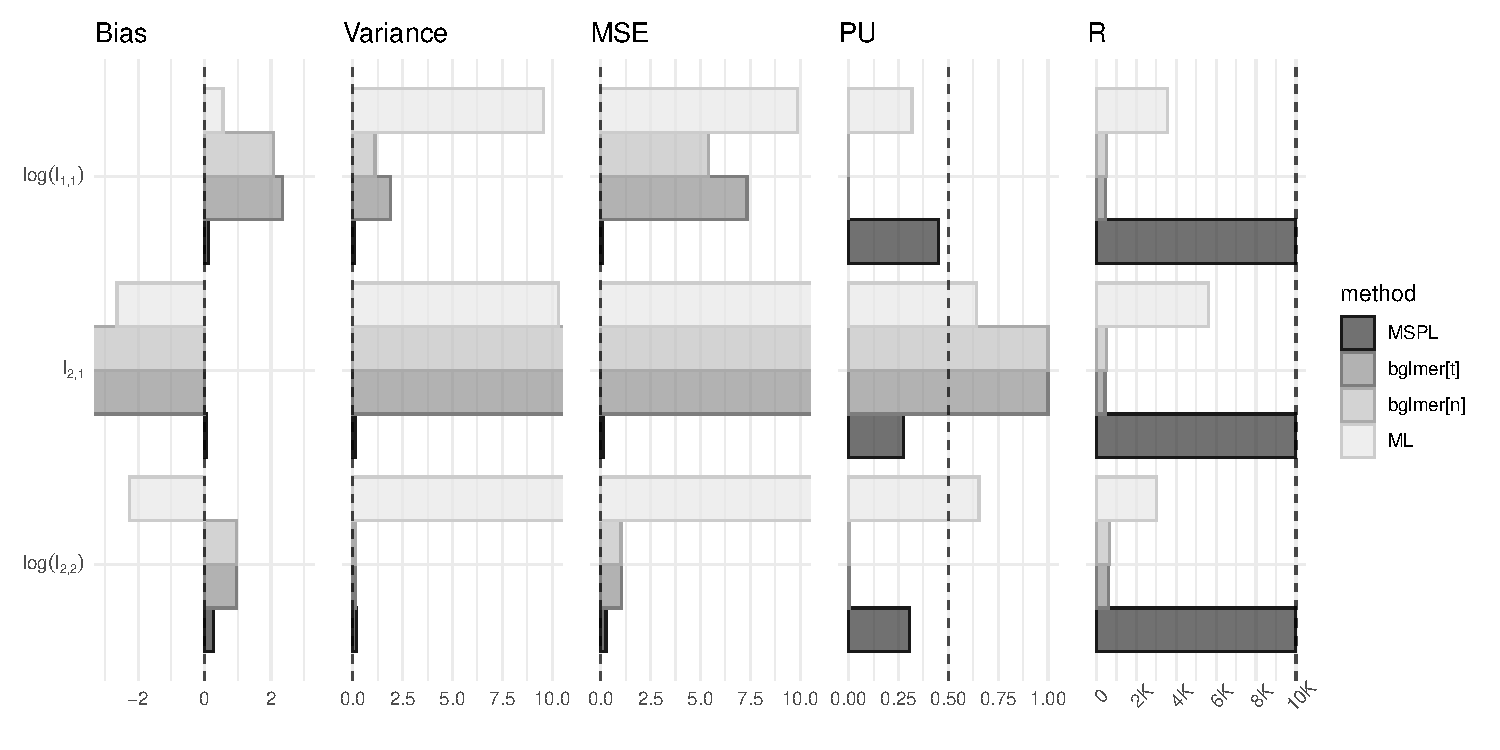
\includegraphics[width=\textwidth]{Figures/cond_inf_simul.pdf}
	\end{center}
	\caption{Performance metrics for variance components estimates of MAL,MSPAL and \texttt{bglmer} from simulating a Bernoulli-response GLMM from the conditional inference data at the MSPAL}
	\label{fig:cond_inf_simul}
\end{figure}

\begin{table}[H]
	\centering
	\caption{Percentiles of centered variance components estimates from simulating a Bernoulli-response GLMM from the conditional inference data at the MSPAL} 
	\label{tab:sim2}
	\begin{tabular}{lrcccccccc}
		\toprule 
		&& \multicolumn{6}{c}{Percentiles} \\ \cmidrule{3-9}
		 &  & 5\% & 10\% & 25\% & 50\% & 75\% &90\% & 95\% \\  
		\cmidrule{3-9}
		& $\log l_{1,1}$ & -0.06 & -0.05 & -0.02 & 0.01 & 0.13 & 0.46 & 0.68 \\ 
		MSPAL & $\log l_{2,2}$ & -0.44 & -0.32 & -0.10 & 0.25 & 0.55 & 0.84 & 0.98 \\ 
		& $l_{2,1}$ & -0.71 & -0.26 & -0.02 & 0.12 & 0.21 & 0.34 & 0.42 \\ \cmidrule{3-9}
		& $\log l_{1,1}$ & 1.03 & 1.09 & 1.30 & 1.79 & 3.89 & 4.64 & 4.95 \\ 
		bglmer(t) & $\log l_{2,2}$ & 0.43 & 0.53 & 0.65 & 0.97 & 1.11 & 1.40 & 1.55 \\ 
		& $l_{2,1}$ & -41.35 & -34.26 & -6.34 & -2.67 & -1.20 & -0.79 & -0.69 \\ \cmidrule{3-9}
		& $\log l_{1,1}$ & 1.24 & 1.36 & 1.79 & 2.03 & 4.51 & 4.91 & 5.12 \\ 
		bglmer(n) & $\log l_{2,2}$ & 0.55 & 0.59 & 0.81 & 1.01 & 1.17 & 1.38 & 1.49 \\ 
		& $l_{2,1}$ & -39.80 & -32.07 & -25.08 & -3.06 & -2.59 & -2.47 & -2.09 \\ \cmidrule{3-9}
		& $\log l_{1,1}$ & -2.48 & -1.80 & -0.40 & 1.24 & 2.36 & 2.61 & 2.66 \\ 
		MAL & $\log l_{2,2}$ & -7.73 & -4.51 & -3.40 & -1.71 & 0.28 & 0.73 & 1.01 \\ 
		& $l_{2,1}$ & -7.49 & -7.19 & -5.95 & -2.45 & 0.52 & 0.80 & 1.06 \\ 
		\bottomrule
	\end{tabular}
\end{table}

\section{Discussion}
\label{sec:sum}
This paper proposed the MSPAL estimator for stable parameter estimation in Bernoulli-response GLMMs. We showed that using a scaled version of Jeffreys prior as fixed effects penalty and the negative Huber loss function as a variance components penalty gives nondegenerate estimates whose finite sample properties are superior to the penalized estimator proposed by \citet{chung+etal:2013}. While particularly relevant for Bernoulli-response GLMMs, the concept of MSPAL is far more general and we expect it to be useful in other settings, such as GLMMs with Binomial or Poisson responses, for which degenerate M(A)L estimates are known to occur. We leave deriving a unified set of conditions and error rates that satisfy the regularity assumptions that we imposed to derive asymptotic properties of the MSPAL to future research. 

%Finally, it is worth pointing out that throughout this study it was assumed that the model was correctly specified, meaning that the true model is contained within the class of models over which estimation is performed. We consider extending the framework of \citet{yu2018asymptotic} regarding model selection in GLMMs under misspecification to our proposed MSPAL so as to develop a softly penalized MAL estimator that is robust under model misspecification a promising avenue for future research.

\bibliographystyle{chicago}
\bibliography{softpen}


\includepdf[pages=-]{softpen_supplementary.pdf}
\end{document}

% Any two distinct random vectors ${\bb Y}_i$ and ${\bb Y}_j$ may share
% random scalar components. We denote the distinct scalar random
% variables by $Z_1, \ldots, Z_m$, and by $G(z_1, \ldots, z_m)$ their
% typically unknown, underlying joint distribution function. In general
% $m \le \sum_{i = 1}^k c_i$, with equality only if
% ${\bb Y}_1, \ldots, {\bb Y}_k$ have distinct components. Let
% ${\bb Y} = ({\bb Y}_1^\top, \ldots, {\bb Y}_k^\top)^\top$, and denote
% by $X$ the set of ${\bb x}_1, \ldots, {\bb x}_k$.


The idea of soft penalization to handle the estimation degeneracies
encountered in the preceding section is remarkably simple and
general. For clarity of presentation, the concent is introduced here
for general maximum likelihood estimation of parametric models.

Consider a sequence $\textbf{y}_n=(y_1, y_2,\ldots,y_n)$ of
observations corresponding to a sequence of random variables
$\textbf{Y}_n=(Y_1,\ldots,Y_{n})$, $Y_i \in \Re^{N_i}$ indexed
by $n$, possibly with a sequence of covariate vectors
$\bx_1,\ldots,\bx_n$, $\bx \in \Re^{M_i}$
for some sequence of constants $N_i,M_i$. For example in the clustered
GLMM, $n$ could denote the number of clusters, $N_i$ the number of
within cluster observations and $\bx_{i}$ the vector of stacked
within cluster random and fixed effects covariates so that
$M_i=N_i(p+q)$. The specifics depend on the considered modelling
assumptions and asymptotic regime and are immaterial for the
development of the methodology. Further assume that $\textbf{Y}_n$ has
a distribution $\mathcal{P}_n=\mathcal{P}_{n,\tnod}$ which comes from
a class of parametric models
$\{\mathcal{P}_{n,\theta}: \theta \in \Theta \}$ with common parameter
$\theta \in \Theta \subseteq \mathbb{R}^p$. It is assumed that the
true model is contained in the parametric family, i.e.
$\tnod \in \Theta$, and that the models admit a log-likelihood
function
$\ell_n(\theta;\textbf{y}_n,\bx_1,\ldots,\bx_n)$. The
dependence of the likelihood on
$n,\textbf{y}_n,\bx_1,\ldots,\bx_n$ is suppressed for
notational convenience. \PS{Are we happy with this setup?}
%Consider a sequence of models $\mathcal{M}_n$ indexed by $n$ and parametrized by a common parameter $\theta \in \Theta \subseteq \Re^d$. That is $\mathcal{M}_n: \Theta \times \mathcal{X}_n \to \Re$, where $\mathcal{X}_n$ is a measurable space of a data generating process of interest \PS{del this last sentence?} Assume these models admit a log-likelihood $\ell(\theta)$, where the dependence on observed data and $n$ is suppressed. For example, in the standard parametric maximum likelihood setting with i.i.d. observations, $\xi_n = (\xi_1,\ldots,\xi_n) \in \mathcal{X}_n = \mathcal{X}_{\otimes n}$ with density $f_\theta: \mathcal{X}\to \Re$, $\mathcal{M}_n = \{ f_{n,\theta}(\xi_n) = \prod_{i=1}^{n}f_\theta(\xi_i)| \xi_i \in \mathcal{X}, \theta \in \Theta  \}$ and  $\ell(\theta) = \sum_{i=1}^{n}\log(f_\theta(\xi_i))$. In GLMMs however, the model density is more complicated and even the indexing variable $n$ may not be uniquely determined so that the more abstract setup is preferable in this setting. 
The maximum likelihood estimator is simply the maximizer of the log-likelihood $\ell(\theta)$ over the parameter space $\Theta$. In the previous section it was shown that the MLE may lie on the boundary of the parameter space, denote it by $\partial \Theta$.

This is easily avoided by introducing a sequence of penalties $P_n(\theta;\textbf{y}_n)$ to the model log-likelihood, which may depend on the observed data. To avoid notational clutter, the dependence of the penalty of $n,\textbf{y}_n$ is omitted henceforth. The penalties are chosen such that for any path of parameters $\theta_r$ indexed by $r \in \Re$ with $\lim\limits_{r \to \infty} \theta_r \in \partial \Theta$ it holds that $\lim\limits_{r \to \infty} P(\theta_r) = -\infty$ for all $n$ with probability one.  Let $\tilde{\theta} = \arg \underset{\theta \in \Theta}{\max} \; \{\ell(\theta) + P(\theta)\}$ be the softly penalized MLE. Then, if there is at least one point $\theta \in \Theta$ such that $\tilde{\ell}(\theta) = \ell(\theta) + P(\theta)>-\infty$, it must hold that $\tilde{\theta}$ lies in the interior of $\Theta$. 

The idea is now to choose a soft penalty whose gradient is sufficiently stochastically bounded so as to preserve the consistency and asymptotic normality that the standard MLE might have. 

%Naturally, the exact stochastic bounds imposed on the penalties depend on the model and the assumptions used to derive the asymptotic properties of the standard MLE. 

\section{Consistency and asymptotic normality of softly penalized MLE} 
\label{sec:ass+res} 

The derivations below are deliberately kept informal to showcase the general mechanics of the large sample behaviour of the softly penalized MLE. A thorough argument with a set of model conditions that guarantee consistency and asymptotic normality is given in the supplementary material. These are not the only conditions that guarantee consistency and asymptotic normality, and these properties are likely to hold under other standard regularity conditions for parametric models. 

In addition to the notation set up in the introductory paragraph of this section,  let $S(\theta) $ be the score function of $\ell(\theta)$, i.e. $S(\theta ) =\nabla \ell(\theta)$, and let $\tilde{S}(\theta)$ be the score of its penalized analogue. Denote the observed information by $J(\theta) = -\nabla \nabla^\top \ell(\theta)$. % and by $\tilde{J}(\theta) \vcentcolon= -\frac{\partial^2 }{\partial \theta \partial \theta^\top} \tilde{\ell}(\theta)$ respectively. 
It is assumed that information regarding the model parameter accumulates at rate $r_n$ in the sense that $r_n^{-1}J(\theta ) \overset{p}{\to} I(\theta)$ as $n \to \infty$ for some positive definite matrix $I(\theta)$ and with respect to some matrix norm $\mnorm{\cdot}$. To measure the discrepancy of various penalized and unpenalized quantities, introduce the following notation. Let $\delta(\theta) = \|\nabla P(\theta)\|$ % and $\gamma(\theta)=\norm{ J(\theta)-\tilde{J}(\theta)}$ 
for some vector norm $\vnorm{\cdot}$, and for $S \subseteq \Theta$ define $\delta^\infty(S)  = \underset{\theta \in S}{\sup} \; \delta(\theta)$ and denote by $B_t(\theta)$ the ball of radius $t$ around $\theta$. %and similarly $\gamma^{\infty}(S)  \vcentcolon= \underset{\theta \in S}{\sup} \; \gamma(\theta)$
%and for any $\tnod \in \Theta$, $t>0$, write $B_t(\tnod) \vcentcolon= \{\theta \in \Theta: \norm{\theta-\tnod }\leq t \}$ for the ball of radius $t$ around $\tnod$.
To prove consistency of a MLE based on the score function, it is typically assumed that $r_n^{-1}S(\theta)$ converges uniformly in probability to some function $S_0(\theta)$, that $S_0(\theta)$ is uniquely maximized at $\tnod$ and that only $\theta$s in the neighbourhood $\tnod$ achieve values $S_0(\theta)$ which are close to $S_0(\tnod)$. By uniform convergence of $r_n^{-1}S(\theta) $ to $S_0(\theta)$ it then follows that $\|S_{0}(\that)\| \leq \underset{\theta \in \Theta}{\sup}\|r_n^{-1}S(\theta)-S_{0}(\theta) \| + r_n^{-1}S(\that)=o_p(1)$. The additional smoothness assumptions then guarantee that for any $\varepsilon>0$ there is a $\gamma>0$ such that $\|S_0(\theta)\|\geq 0$ implies $\|\theta-\tnod\| \geq \varepsilon$. This establishes consistency as it was argued that $\|S_0(\that)\|=o_p(1)$.

Now to amend this reasoning to the softly penalized MLE, assume that $\delta(\ttilde) = o_p(r_n)$. Then by construction $r_n^{-1}{S}(\ttilde) = -r_n^{-1}\delta(\ttilde) = o_p(1)$. But then it is also the case that $\|S_0(\ttilde) \|= o_p(1)$ and consistency is achieved under the same conditions as for the ordinary MLE if the gradient of the penalty decays at a stochastic rate faster than $r_n$. Note that the same argument applies when in place of the exact likelihood $\ell(\theta)$, one considers an approximate likelihood, for which the error in the approximation to the score function is of the same stochastic order as the gradient of the soft penalty, namely $o_p(r_n^{-1})$. The exact regularity conditions to motivate Theorem \ref{thm:soft_pen_cons}, which are classic model regularity conditions in M-estimation \citep[Theorem 5.9]{vaart1998asymptotic}, are given in the supplementary material along with the proof of the theorem. 
%\begin{enumerate}[label = A\arabic*)]
%	\item Both $\ell(\theta),\tilde{\ell}(\theta)$ are differentiable, with derivatives $S(\theta),\tilde{S}(\theta)$ 
%	\item $\underset{\theta \in \Theta}{\sup} \; \norm{r_n^{-1} S(\theta) - S_0(\theta)} \overset{p}{\to}0$ for some function $S_0(\theta)$ 
%	\item For all $\varepsilon>0$, $\underset{\theta \in \Theta: \norm{\theta-\tnod}\geq \varepsilon}{\inf} \norm{S_0(\theta) }>0 = \norm{S_0(\tnod)}$ 
%	\item $\ttilde$ is an (approximate) root of $\tilde{S}(\theta)$ such that $r_n^{-1}\tilde{S}_n(\ttilde) = o_p(1)$
%\end{enumerate}
\begin{theorem}[Consistency of the softly penalized MLE]
	\label{thm:soft_pen_cons}
	Let $\delta(\ttilde) =   o_p(r_n)$. Then $\ttilde$ is consistent for $\tnod$.  
\end{theorem}
%\begin{proof}
%	The proof follows \cite[Thm. 5.7 \& 5.9]{vaart1998asymptotic}. First, consider the distance from  $r_n^{-1}\tilde{S}(\ttilde)$ to $S(\ttilde)$: 
%	\begin{equation}
%	\label{eq:soft_pen_cons_proof_1}
%	\begin{aligned}
%	r_n^{-1}S(\ttilde) & = r_n^{-1}\tilde{S}(\ttilde) + r_n^{-1}(S(\ttilde)-\tilde{S}(\ttilde)) \\
%	&= r_n^{-1}\tilde{S}(\ttilde) +r_n^{-1}\frac{\partial }{\partial \theta} P(\ttilde) \\
%	&= o_p(1) +r_n^{-1}\frac{\partial }{\partial \theta} P(\ttilde)
%	\end{aligned}
%	\end{equation}
%	where the second equality follows from the definition of $\tilde{l}(\theta) = \ell(\theta) + P(\theta)$ and the last equality comes from A4). Hence, $\ttilde$, in connection with A1-A3, satisfies the conditions of Theorem 5.9 in \cite{vaart1998asymptotic}, which guarantees consistency. In particular, note that by \eqref{eq:soft_pen_cons_proof_1} and A4), $\norm{r_n^{-1}{S}(\ttilde)} =   o_p(1)$. Adding $\norm{S_0(\ttilde)}$ to both sides of this equation and rearranging yields 
%	\begin{equation}
%	\label{eq:soft_pen_cons_proof_2}
%	\begin{aligned}
%	\norm{S_0(\ttilde)}&=   \norm{S_0(\ttilde)}-\norm{r_n^{-1}{S}(\ttilde)} + o_p(1) \\ 
%	&\leq \underset{\theta \in \Theta}{\sup} \norm{r_n^{-1}{S}(\theta)-S_0(\theta) } + o_p(1)  \\ 
%	&= o_p(1)	
%	\end{aligned}
%	\end{equation}
%	where the second line follows from the reverse triangle inequality and the  third from \eqref{eq:soft_pen_cons_proof_1} and A2). Finally note that A3 implies that for any $\varepsilon>0$, there is a number $\eta$ such that $\norm{S_0(\theta)}>\eta$ for any $\theta: \norm{\theta-\tnod}\geq \varepsilon$. Hence, for any $\varepsilon>0$, the event $\norm{\ttilde-\tnod}\geq \varepsilon$ is implied by the event $\norm{S_0(\ttilde)}>\eta$, however, this was seen to converge to zero in probability in \eqref{eq:soft_pen_cons_proof_2}.
%\end{proof}
%The similarity of the conditions of theorems \ref{thm:extremum} and \ref{thm:asymp_norm_soft_pen} is immediate and illustrates that many variations on the general theme of proving consistency for extremum estimators lead to the same result – and thus consistency of the softly penalized MLE. \\ 

To establish asymptotic normality of the softly penalized MLE, a simple stochastic Taylor expansion suffices as the informal argument below demonstrates. Following the notational convention introduced before, a Taylor expansion of the score around the MLE yields 

\begin{equation}
\label{eq:asymp_norm_taylor_1}
\begin{aligned}
S(\theta) = S(\that) + \nabla S(\theta) \big|_{\theta = \theta^*} (\theta-\that) 
= -J(\theta^*) (\theta-\that) 
\end{aligned}
\end{equation}
where $\theta^*$ lies in a ball of radius $\|\theta-\that\| $ around $\that$ and  $J(\theta^*) = -\nabla^\top \nabla \ell(\theta) |_{\theta = \theta^*}$. Now by construction $\tilde{S}(\theta) -S(\theta) =\nabla P(\theta)$, and it follows that for $\ttilde$, such that $\tilde{S}(\ttilde) = 0$, 

\begin{equation}
\label{eq:asymp_norm_taylor_2} 
0 = \tilde{S}(\ttilde) = -J(\theta^*) (\ttilde-\that) + \nabla P(\ttilde)
\end{equation}
so that 
\begin{equation}
\label{eq:asymp_norm_taylor_3}
\ttilde-\that = [r_n^{-1}J(\theta^*)^{-1} ][r_n \nabla P(\ttilde)]
\end{equation}
On the other hand trivially 
\begin{equation}
r_n^{1/2}(\ttilde-\tnod) = 	r_n^{1/2}(\that-\tnod) +	r_n^{1/2}(\ttilde-\that)
\end{equation}
If, as is typical for MLEs, it is the case that $ r_n^{-1} J(\theta) \overset{p}{\to} I(\theta)$ uniformly over $\Theta$, and $r_n^{1/2}(\that-\tnod) \overset{d}{\to}\text{N}(0,I(\tnod)^{-1})$, as $n \to \infty$, for some index $n$ and some rate of information accumulation $r_n$, then, assuming consistency of $\ttilde$, $r_nJ(\ttilde)^{-1} \overset{p}{\to} I(\tnod)$. Hence to achieve asymptotic normality, all that is needed is 
\begin{equation}
	\nabla P(\ttilde) = o_p(r_n^{1/2})
\end{equation}
%A possible way to achieve this is to find a penalty whose gradient is uniformly $o_p(r_n^{1/2})$ over the whole parameter space or in a neighbourhood around $\tnod$. 
%\begin{enumerate}[label=B\arabic{*})]
%	\item Both $\ell(\theta),\tilde{\ell}(\theta)$ are twice differentiable
%	\item $\underset{\theta \in \Theta}{\sup}\; \norm{ r_n^{-1}J(\theta) -I(\theta) } \overset{p}{\to} 0$ for some positive definite matrix $I(\theta)$, which is continuous in $\theta$ in a neighbourhood around $\tnod$
%	%	\item $\that \overset{p}{\to}  \tnod$ 
%	\item $r_n^{1/2}(\that-\tnod) \overset{d}{\to} \text{N}(0,I(\tnod)^{-1})$
%	\item[(B4)] $\ttilde$ is consistent for $\tnod$. 
%\end{enumerate}

%Note that assumption B2, which appears to be the strongest of the four, is a standard condition to prove B3. B4 can be treated as a separate assumption, alternatively, conditions A1-A4 can be included. 

From the argument above it follows immediately that if $\delta^\infty(\Theta)=o_p(r_n^{1/2})$, then $r_n^{1/2}(\that-\tnod) \overset{d}{\to}\text{N}(0,I(\theta)^{-1})$, as $n \to \infty$. An auxiliary lemma due to \cite{ogden:2017}, which is given in the supplementary material, can be used relax the uniformly boundedness condition on the gradient of the penalty to a neighbourhood around $\tnod$. Note again that if one considers an approximate log-likelihood, whose approximation error to the score is uniformly $o_p(r_n^{1/2})$ (in a neighbourhood of $\tnod$), the same argument applies. 

The supplementary material provides a concise set of assumptions that are sufficient to formalize the above argument along with the proof of Theorem \ref{thm:asymp_norm_soft_pen}. 

%\begin{lemma}
%	\label{lemma:ogden}
%	Suppose that $\delta(\ttilde) =    o_p(r_n)$ and that there is a $t>0$ such that $\delta^{\infty}(B_t(\tnod)) = o_p(a_n)$ for some nonnegative sequence $a_n$ indexed by $n$. Then $\ttilde-\tnod=o_p(a_nr_n^{-1})$. 
%\end{lemma}
%\begin{proof}
%	The proof is similar to \cite[Lemma 1]{ogden:2017}.
%	A first order Taylor expansion of $S(\theta)$ around $\that$ yields 
%	\begin{equation}
%	\label{eq:lemma_ogden_proof_1}
%	\begin{aligned}
%	S(\theta) = S(\that) + \frac{\partial S(\theta)}{\partial \theta^\top} \bigg|_{\theta = \theta^*} (\that-\theta) 
%	= -J(\theta^*) (\theta-\that) 
%	\end{aligned}
%	\end{equation}
%	where $\theta^*$ lies between $\that$ and $\theta$. 
%	
%	Now letting $\nabla_\theta \epsilon(\theta) =  \tilde{S}(\theta) -S(\theta)$, it follows that for $\ttilde$, such that $\tilde{S}(\ttilde) = 0$, 
%	
%	\begin{equation}
%	\label{eq:lemma_ogden_proof_2} 
%	0 = \tilde{S}(\ttilde) = -J(\theta^*) (\ttilde-\that) + \nabla_\theta \epsilon(\ttilde)
%	\end{equation}
%	so that 
%	\begin{equation}
%	\label{eq:lemma_ogden_proof_3}
%	\ttilde-\that = [r_n^{-1}J(\theta^*)]^{-1} r_n^{-1}\nabla_\theta \epsilon(\ttilde)
%	\end{equation}
%	for some $\theta^*$ between $\that$ and $\ttilde$. Now by B4 or Theorem \ref{thm:soft_pen_cons}, $\ttilde$ is consistent so that also $\theta^*$ is consistent. Hence by assumption B2, it follows that  $[r_n^{-1}J(\theta^*)]^{-1}$ converges in probability to $I(\tnod)^{-1}$ so that $\ttilde-\that = \Op{r_n^{-1}\delta(\ttilde)}$. 
%	
%	Now let $A_n = \{\ttilde \in B_t(\tnod) \}$ for the $t$ such that $\delta^{\infty}(B_t(\tnod)) = o_p(a_n)$ for some nonnegative sequence $a_n$ indexed by $n$. Then, by construction, conditional on $A_n$, $\ttilde-\that = \Op{r_n^{-1}\delta^\infty(B_t(\tnod))} = o_p(r_n^{-1}a_n)$. Moreover, since $\ttilde$ is consistent, $\Pr(A_n) \to 1$ as $n\to \infty$. Putting everything together, one gets that for any $\varepsilon>0$, 
%	\begin{equation}
%	\label{eq:lemma_ogden_proof_4} 
%	\begin{aligned}
%	\Pr\left(\norm{\ttilde-\tnod}\geq \varepsilon r_n^{-1}a_n\right) & = \Pr\left(\norm{\ttilde-\tnod}\geq \varepsilon r_n^{-1}a_n|A_n\right)\Pr(A_n)\\ &+ 
%	\Pr\left(\norm{\ttilde-\tnod}\geq \varepsilon r_n^{-1}a_n|\bar{A}_n\right)\Pr(\bar{A}_n) \\
%	&\leq \Pr\left(\norm{\ttilde-\tnod}\geq \varepsilon r_n^{-1}a_n|A_n\right) + \Pr(\bar{A}_n) \to 0, \quad n \to \infty
%	\end{aligned}
%	\end{equation}
%	as required. 
%\end{proof}
%An immediate consequence of this lemma and assumptions B1-B4 is the following theorem. 

\begin{theorem}[Asymptotic Normality of the softly penalized MLE]
	\label{thm:asymp_norm_soft_pen}
	Let $\delta(\ttilde) =   o_p(r_n)$ and assume there is a $t>0$ such that $\delta^{\infty}(B_t(\tnod)) = o_p(r_n^{1/2})$. Then 
	$r_n^{1/2}(\ttilde-\tnod) \overset{d}{\to} \text{N}(0,I(\tnod)^{-1})$. 
\end{theorem} \vspace{.5cm}
%\begin{proof}
%	By Lemma \ref{lemma:ogden}, it holds that $\ttilde-\that = o_p(r_n^{-1/2})$ so that $r_n^{1/2}(\ttilde-\tnod) = r_n^{1/2}(\that-\tnod)+r_n^{1/2}(\ttilde-\that) = r_n^{1/2}(\that-\tnod) + o_p(1)$ and the result follows by B4. 
%\end{proof}

If it is additionally assumed that $\underset{\theta \in B_t(\tnod)}{\sup} \mnorm{\nabla\nabla^\top P(\theta)}=o_p(r_n)$, then < shows that under the null $H_0: \tnod \in \Theta_R$, where $\Theta_R$ is some subspace of $\Theta$ of strictly lower dimension than $\Theta$, the penalized likelihood ratio $\tilde{\Lambda} = 2 \{\tilde{\ell}(\ttilde)- \tilde{\ell}(\ttilde_R)\}$, where $\ttilde_R$ is the penalized maximum likelihood estimate restricted to $\Theta_R$, is asymptotically equivalent to the unpenalized likelihood ratio. Hence, this result provides asymptotically valid inference based on likelihood ratios or Wald and score test statistics. The supplementary material gives bounds on the Hessians of the penalties employed in this paper, which, upon determination of $r_n$, can be used to justify hypothesis testing. \PS{or give in paper? }

This section concludes with two remarks. The conditions under which the asymptotic properties of the softly penalized MLE were derived are one of many, and as long as the log-likelihood $\ell(\theta)$ and the penalty $P(\theta)$ are sufficiently smooth, arguments that are similar in spirit to those given in this section, are expected to apply. Moreover, the results presented in this section, which can be seen as establishing the asymptotic properties of the maximizer of an approximate likelihood, immediately give conditions on the approximation error of the numerical approximation to the score of \eqref{eq:bern_likl} that ensure consistency and asymptotic normality of the resulting estimator. 
%Hence, if such a bound on the approximation error is known, it is an easy task to generalize the results of this section to the MLE of the numerical approximation to the likelihood \eqref{eq:bern_likl} through a suitably chosen sequence of quadrature points. 

\subsection{Penalty scaling factors}
\label{sec:scaling} 

The conditions of Theorems \ref{thm:soft_pen_cons} and \ref{thm:asymp_norm_soft_pen} on the penalty function can be dissected into a (uniform) boundedness condition on the gradient of the penalty and a rate requirement. Hence, a straightforward strategy to select penalties is to first find an unscaled penalty function $P_u(\theta)$  such that for any path of parameters $\theta_r$ indexed by $r \in \mathbb{R}$ with $\lim\limits_{r \to \infty} \theta_r \in \partial \Theta$ it holds that $\lim\limits_{r \to \infty} P_u(\theta_r) = -\infty$. Then, upon determining suitable stochastic bounds for the gradient of the penalty, one can rescale the penalty function accordingly to achieve consistency and asymptotic normality. \\ 

The scaling factors in this paper are based on
\begin{equation}
 \frac{1}{4p}\mnorm{\bX^\top\bX}_{1} = \frac{1}{4p}	\sum_{i=1}^{p} \sum_{j=1}^{n}x_{ji}^2 
\end{equation}
 where $\mnorm{\cdot}_{1}$ denotes the Schatten 1-norm. An adaptation of the proof of Theorem 2)i) of \citet{kosmidis+firth:2020}, which is given in the supplementary material, shows that $\frac{1}{4}\mnorm{\bX^\top\bX}_{1}$ maximizes the Schatten 1-norm of the information from a standard logistic regression model with respect to $\beta \in \Re^p$. The factor $1/p$ is added so that the scaling factor captures so as to normalize the scaling factor over the number of covariates. As is shown in Theorem \ref{thm:jeffrey_deriv_bound}, scaling the proposed fixed effects penalty, the logarithm of Jeffreys invariant prior from a logistic GLM, by $\mnorm{\frac{1}{4p}\bX^\top\bX}_{1}^{-1/2}$ is sufficient to meet the requirements of Theorems \ref{thm:soft_pen_cons} and \ref{thm:asymp_norm_soft_pen} as long as the rate of information accumulation $r_n$ is monotonically increasing with the indexing sequence $n$. \PS{Insert simulation evidence in favor of scaling by sqrt here.} \\ 


%This amounts to $\lim\limits_{\bL\to \textbf{0}_{q \times q}} \mnorm{[J(\textbf{0}_p,\bL)]_{\beta,\beta}}_{1}$, where $[J(\beta,\bL)]_{\beta,\beta}$ is the $p \times p$ submatrix of the observed information that corresponds to its fixed effects components and $J(\beta,\bL)$ is the negative Hessian of the model log-likelihood evaluated at $\beta,\bL$. Note that $\frac{1}{4}\bX^\top\bX$ is the Fisher-information of a Bernoulli-response GLM with logistic link evaluated at $\beta = \textbf{0}_p$. An adaptation of the proof of Theorem 2)i) of \citet{kosmidis+firth:2020}, which is given in the supplementary material \PS{make!} shows that the nuclear norm of the logistic GLM Fisher information, denote it by $\mnorm{ \bX^\top\bW(\beta)\bX }_{1}$, where $[\bW]_{ii} = \mu_i(1-\mu_i), \mu_i=\textrm{logit}^{-1}(\bx_i^\top\beta)$, is maximized at $\beta = \textbf{0}_p$. 
%A sequence of scaling factors, which conveniently applies under any asymptotic regime in which $r_n^{-1}J(\theta) \overset{p}{\to} I(\theta)$ for any $\theta \in \Theta$ is given by the appropriately scaled norm of the observed information matrix. 
%
%To illustrate the idea, assume that $\nabla P_u(\ttilde) = o_p(r_n^{\alpha})$ for some $\alpha \in \Re$. Now consider rescaling the penalty by $\mnorm{J(\bar{\theta})}^{\kappa}$, where $\bar{\theta}$ is any point in the parameter space such that $\|J(\bar{\theta})\| \neq 0$ and $\kappa \leq 1-\alpha$. It is straightforward to show that  $\mnorm{r_n^{-1}J(\theta)-I(\theta)} = o_p(1)$, implies that $\mnorm{J(\theta)} = O_p(r_n)$. 
%% $\norm{I(\theta)}=\mathcal{O}(1)$, so it follows that $\norm{r_n^{-1}J(\theta)} = \mathcal{O}_p(1)$. By the triangle inequality, $\norm{r_nJ(\theta)} \leq \norm{I(\theta)} + \norm{r_n^{-1}J(\theta)-I(\theta)}$. And hence $\Pr(\norm{r_nJ(\theta)}>\delta) \leq \Pr(\norm{r_n^{-1}J(\theta)-I(\theta)}>\delta-\norm{I(\theta)})$, which goes to zero for any $\delta >\norm{I(\theta)}$ so that by definition $\norm{r_n^{-1}J(\theta)} = \Op{1}$ and thus $\norm{J(\theta)} = \Op{r_n}$.
%Hence, the rescaled penalty $P(\theta) =  \mnorm{J(\bar{\theta})}^{\kappa}P_u(\theta)$ is $o_p(r_n)$ for any fixed $\bar{\theta} \in \Re^p$. To meet the requirements for asymptotic normality, assume that $\nabla P_u(\ttilde) = o_p(r_n^{\alpha})$ and additionally that for some $t>0$, $\underset{\| \theta-\tnod\|<t}{\sup} \nabla P_u(\theta) = o_p(r_n^{\gamma})$ for some $\gamma \in \Re$. Then rescaling $P_u(\theta)$ by $\mnorm{J(\bar{\theta})}^{\kappa}$ for any $\kappa \leq \min \{ 1-\alpha, \frac{1}{2}-\gamma\}$ ensures that the rescaled penalty meets the requirements of Theorems \ref{thm:soft_pen_cons} and \ref{thm:asymp_norm_soft_pen}.   \\ 
%
%The choice of admissible norms depends on the norm that establishes convergence of $r_n^{-1}J(\theta)$. For concreteness, consider the nuclear norm. As the nuclear norm is the Schatten 1-norm, it follows from the monotonicity of the Schatten p-norms, that for any $p\geq 1$, $\mnorm{J(\theta)}_1 \geq \mnorm{J(\theta)}_p$. Hence, nonregarding the Schatten p-norm used to motivate $r_n^{-1}J(\theta) \overset{p}{\to} I(\theta)$, it is guaranteed that $\mnorm{J(\bar{\theta})}_1^{-1} J(\theta) \leq \mnorm{J(\bar{\theta})}^{-1}_pJ(\theta) = \Op{1}$ so that always $\mnorm{ J(\that)}^{-1} = \Op{r_n^{-1}}$. \\ 

%If it moreover holds that convergence of the observed information $J(\theta)$ is uniform over the parameter space and that for some sequence of parameters $\bar{\theta}_n$, $\lim\limits_{n \to \infty} \bar{\theta}_n = \bar{\theta}$, $\norm{I(\bar{\theta})}<\infty$, then it holds that $\norm{J(\bar{\theta}_n)}=\Op{r_n}$. In this instance, defining $\bar{\theta}_n$ as the unpenalized MLE $\that$, whenever it exists, and setting it to an arbitrary but fixed value $\theta$ for which $\|J({\theta})\|\neq 0$ otherwise, gives a the natural scaling factor $\| J(\bar{\theta}_n)\|^{\kappa}$ with $\kappa \leq \min \{1-\alpha, \frac{1}{2}-\gamma \}$ as before. \\ 
%$I(\theta)$ is continuous in $\theta$ around $\bar{\theta} $ and

%To illustrate this point, recall that for consistency of the softly penalized MLE, it was required that the first derivative of the penalty at the softly penalized MLE must be of stochastic order strictly smaller than $r_n$, that is $\frac{\partial}{\partial \theta} P_u(\theta) = o_p(r_n)$ and that for asymptotic normality, it was required that at least in a neighbourhood around the true $\tnod$, $\frac{\partial}{\partial \theta} P(\theta) = o_p(r_n^{1/2})$. Hence, if the first derivative of a candidate penalty is known to be uniformly $o_p(r_n)$, that is $\underset{\theta \in \Theta}{\sup} \frac{\partial}{\partial \theta} P_u(\theta) = o_p(r_n)$. Then rescaling this penalty by $\| J(\theta_n) \|^{-1/2}=\Op{r_n^{-1/2}}$ gives a penalty that satisfies the conditions of theorems \ref{thm:soft_pen_cons} \& \ref{thm:asymp_norm_soft_pen}.  

%As Theorems \ref{thm:soft_pen_cons} and \ref{thm:asymp_norm_soft_pen} only require the gradient of the penalty function to be of stochastic order no greater than $r_n$ and $r_n^{1/2}$ respectively, there are naturally infinitely many possible scaling factors that satisfy these requirements for any suitably bounded penalty function. For example, the real-data examples in this paper give rise to $\Op{1}$ gradients of the fixed effects penalty and the variance components penalty, so that for the proposed scaling factor $\mnorm{J(\bar{\theta})}^\kappa$, any $\kappa \in (-\infty,1)$ achieves consistent estimates and $\kappa \in (-\infty,1/2)$ achieves asymptotically normally distributed estimates. Figure \ref{fig:culcita_scale} demonstrates the shrinkage of the softly penalized MLE on both the full Culcita dataset and the degenerate subdataset, where the scaling factor $\mnorm{J(\bar{\theta})}^\kappa$ is varied over powers $\kappa$. The grey-shaded area indicates scalings that preserve consistency only. For scalings where asymptotic normality is preserved, the pointwise asymptotic 95\% confidence intervals are shaded in blue. Degenerate estimates were given unbounded confidence intervals. \PS{Comment about this?}   
%


%In this study it was found that for penalties with $\Op{1}$ derivatives, a scaling by $\|J(\bar{\theta})\|^{-1/2}$ has given the best compromise between stable estimation and adequate parameter recovery. \PS{Comment about shrinkage? Not sure what we want here} 


%
%\begin{figure}[H]
%	\begin{subfigure}[t]{\textwidth}
%		\includegraphics[width=\textwidth]{Figures/Culcita/culcita_scale_full.pdf}
%		\caption{Full data}
%	\end{subfigure}
%	\begin{subfigure}[t]{\textwidth}
%		\includegraphics[width=\textwidth]{Figures/Culcita/culcita_scale_deg.pdf}
%		\caption{Degenerate subdata}
%	\end{subfigure}
%	\caption{Dependence of the softly penalized MLE on the exponent $\kappa$ of the adapative scaling factor $\mnorm{J(\bar{\theta})}^{\kappa}$. Estimate come from fitting a clustered logistic regression model with random intercepts to the Culcita dataset.}
%	
%	\label{fig:culcita_scale}
%\end{figure}

%\begin{figure}[H]
%	\label{fig:culcita_scale_full_no_ci}
%	\includegraphics[]{Figures/Culcita/culcita_scale_full_no_ci.pdf}
%	\caption{Dependence of the softly penalized MLE on the exponent $\beta$ of the adapative scaling factor $\|J(\bar{\theta})\|^\beta$ resulting from fitting a clustered logistic regression model with random intercepts to the Culcita dataset.}
%\end{figure}

%Several variations of this theme are possible. The point to stress is that under the conditions of \ref{thm:asymp_norm_soft_pen}, $\|J(\that)\| = \Op{r_n}$ which can be used to conveniently scale any potential penalty to meet the requirement of theorems \ref{thm:soft_pen_cons} \& \ref{thm:asymp_norm_soft_pen}.  

\subsection{Fixed effects penalty} 
\label{sec:penalties} 

The unscaled fixed effects penalty considered in this study is $P_u^{\text{FE}}(\beta) =  \frac{1}{2}\log \det(\bX^\top\bW\bX)$. Here $\bX$ is the matrix of all fixed effect covariates, $\bW$ is a diagonal matrix with diagonal entries $\bW_{ii} = \mu_i(\beta) (1-\mu_i(\beta))$ and $\mu_i(\beta)$ is the inverse logit-transform of the fixed effects component of the linear predictor at a point $\beta$ in the parameter space, i.e. $\textrm{logit}(\mu_i(\beta))= \textbf{\bx}_i^\top\beta$. For notational convenience, the dependence of $\mu(\beta)$ on $\beta$ is henceforth suppressed. This penalty function, which is the logarithm of Jeffreys invariant prior for a binomial-response GLM, has a long tradition in the bias reduction literature for maximum likelihood estimators \citep{firth1993bias,kosmidis+firth:2020}. Recently, \citet[Theorem 1]{kosmidis+firth:2020} have shown that whenever $\bX$ is full rank, then for any sequence $\beta_r \in \Re^p$ indexed by $r \in \Re$ such that $\lim\limits_{r \to \infty} \underset{1\leq i \leq p}{\min} |\beta_r^{(i)}| = \infty$, $\lim\limits_{r \to \infty} \det(\bX^\top\bW\bX) = 0$, where $\beta_r^{(i)}$ refers to the $i${th} component of $\beta_r$. Therefore, noting that \eqref{eq:bern_likl} is always bounded from above by one as the conditional distribution of the response is a probability mass function, adding this penalty to the log-likelihood guarantees finite fixed effect parameter estimates as long as there is one $\theta \in \Theta$ for which the log-likelihood is not $-\infty$. The logistic link in Jeffreys prior penalty appears sensible for the clustered logistic regression model with random intercepts, which can be interpreted as penalizing extreme contributions of certain fixed effects covariates to the conditional mean. But as \citet{kosmidis+firth:2020} show, the finiteness property of the (softly) penalized MLE when penalizing with Jeffreys invariant prior extends to other link functions. In particular, if the inverse logistic function, denote it by $G(\eta) = \frac{e^\eta}{1+e^\eta}$, is replaced by any twice differentiable, invertible function $G: (0,1) \to \Re$, then the expected information matrix that would result from a Bernoulli-response GLM under said link, is again of the form $\bX^\top\bW\bX$, where now $w_{ii} = \omega({\eta}_i)$ with $\omega(\eta) = \frac{G'(\eta)^2}{G(\eta)(1-G(\eta))}$, $G'(\eta) = \frac{d G(\eta)}{d \eta}$ and ${\eta}_i = \bx_{i}^\top\beta$. If it is the case that $\underset{|\eta|\to \infty}{\lim} \omega(\eta)=0$, then \citet{kosmidis+firth:2020} show that it still holds that $\lim\limits_{r \to \infty} \det(\bX^\top\bW\bX)=0$, for any sequence $\beta_r \in \Re^p$ indexed by $r \in \Re$ such that $\lim\limits_{r \to \infty} \underset{1\leq i \leq p}{\min} |\beta_r^{(i)}| = \infty$. Specifically, the logit, probit, complementary log-log, log-log and cauchit links are some commonly-used link functions for which $\underset{|\eta|\to \infty}{\lim} \omega(\eta)=0$.

%\IK{Add paragraph about exactly invariant under linear transformations}
Besides the above described limiting behaviour, which makes the logarithm of Jeffreys invariant prior a natural fixed effects penalty, it is also known to be invariant under linear transformations. This invariance property is attractive for applied work as it preserves the property that the MLE of the difference of two (or more) fixed effects components is simply the difference of their MLEs. \PS{Throw out previous sentence?}

All that remains is to determine the appropriate scaling factor of the fixed effects penalty. 
%
%For this, consider the gradient of the unscaled penalty with respect to $\beta$, for which the conditions in Theorems \ref{thm:soft_pen_cons} and \ref{thm:asymp_norm_soft_pen} are formulated. The first partial derivative of the fixed effects penalty with respect to $\beta_i$ is given by
%
%\begin{equation}
%\label{eq:deriv_jeffr_prior}
%\frac{\partial\log \det(\bX^\top\bW\bX) }{\partial \beta_i} = \textrm{tr}\left( (\bX^\top\bW\bX)^{-1}\bX^\top\bW\widetilde{\bW}_i\bX \right) % , \quad 
%%\widetilde{\bW}_i =\textrm{diag}((1-2\mu)\bX_{\cdot,i}) 
%\end{equation}
%
%where $\widetilde{\bW}_i$ is a diagonal matrix with diagonal entries  $[\widetilde{\bW}_i]_{jj}=(1-2\mu_j)[\bX]_{ji}$. In the simplest case where $\beta \in \Re$ is just an intercept, it is easily verified that \eqref{eq:deriv_jeffr_prior} simplifies to $1-2\mu$, where $\textrm{logit}(\mu)=\beta$ which lies in $[-1,1]$ for $\beta \in \Re$. Hence scaling $P_u^{\text{FE}}(\beta)$ by any sequence $\lambda_n = o_p(r_n^{1/2})$ results in a penalty that satisfies Theorems \ref{thm:soft_pen_cons} and \ref{thm:asymp_norm_soft_pen}. 
The theorem below, a proof of which is given in the supplementary material, bounds the gradient of Jeffreys invariant prior for general $\bX \in \Re^{n \times p}, \beta \in \Re^{p}$ and shows that the scaled fixed effects penalty is appropriate for Theorems \ref{thm:soft_pen_cons} and \ref{thm:asymp_norm_soft_pen}.

\begin{theorem}[Bounding the derivative of the log of Jeffreys invariant prior]
	\label{thm:jeffrey_deriv_bound}
	Let $\bX\in \Re^{n \times p}$ be a full column rank matrix, $\bW$ a diagonal matrix with entries $w_j=[\bW]_{jj} = \mu_j(\beta)(1-\mu_j(\beta))$ and $\textrm{logit}(\mu_j(\beta)) = \bx_{j}^\top\beta$ $\beta \in \Re^p$. Then 
	\begin{equation}
	\left|\frac{\partial\log \textrm{det}(\bX^\top\bW\bX) }{\partial \beta_i}\right|  \leq p\underset{1\leq j\leq n}{\max} |x_{ji}(1-2\mu_j(\beta))| \leq p\underset{1\leq j\leq n}{\max} |x_{ji}|
	\end{equation}
	and letting $\mnorm{\cdot}_1$ be the Schatten 1-norm, and for $\bx\in \Re^p$, $\|\bx \|_q =\left(\sum_{i=1}^{p}x_i^q\right)^{1/q}$, $q \in [0,\infty]$, it holds that 
	\begin{equation}
	\mnorm{\bX^\top\bX}_1^{-1/2} \|\nabla\log \textrm{det}(\bX^\top\bW\bX) \|_q \leq p^{\frac{q+1}{q}}
	\end{equation}
\end{theorem}

Note that this bound holds pointwise for any $\beta \in \Re^p$ and uniformly over a ball of arbitrary but finite radius $t$ around any $\beta_0 \in \Re^p$. Although not the sharpest bound possible it is sufficient to meet the criteria of Theorems \ref{thm:soft_pen_cons} and \ref{thm:asymp_norm_soft_pen} as long as $r_n$ is monotonically increasing in $n$. 

%In line with Section \ref{sec:scaling}, the penalty is scaled by the inverse of squareroot of the nuclear norm of the observed information matrix evaluated at the ordinary MLE $\that$, so it exists.

% \PS{Throw out:Since the nuclear norm is the Schatten 1-norm, it follows by the monotonicity of the Schatten p-norms, that for any $p\geq 1$, $\norm{J(\theta)}_1 \geq \norm{J(\theta)}_p$. Hence, nonregarding the Schatten-norm used to motivate $r_n^{-1}J(\theta) \overset{p}{\to} I(\theta)$, it is guaranteed that $\norm{J(\that)}_1^{-1} J(\theta) \leq \norm{J(\that)}^{-1}_pJ(\theta) = \Op{1}$ so that always $\| J(\that) \|^{-1} = \Op{r_n^{-1}}$. }

%The simulations in this study have shown that scaling the fixed effects penalty by $\|J(\that)\|^{-1/2}$ provide a good compromise between strong enough penalization to ensure stable maximum likelihood estimation and effective parameter recovery. 




\subsection{Variance components penalty} 
\label{sec:pen_re}

The variance components penalties considered in this study are simpler than the fixed effects penalty and somewhat ad-hoc, as they do not depend on the observed data apart from the scaling factor that ensures the asymptotic negligibility of the penalty. For simplicity, assume first that the random effects are i.i.d. draws from a univariate normal distribution with standard deviation $\sigma \in \Re_{>0}$. Following the results of Section \ref{sec:ass+res}, a variance components penalty $P^{\text{RE}}(\sigma)$ on $\sigma$ must satisfy the following properties: 
\begin{enumerate}
	\item $\underset{|\log(\sigma)| \to \infty }{\lim} \; P^{\text{RE}}(\sigma) = -\infty$
	\item $\nabla P^{\text{RE}}(\tilde{\sigma}) = o_p(r_n)$
%	, where the notation of Section \ref{sec:ass+res} applies. 
	\item $\underset{\sigma: |\sigma-\sigma_0|\leq t}{\sup} \; \nabla P^{\text{RE}}({\sigma}) = o_p(r_n^{1/2})$ for some $t>0$. 
\end{enumerate}
and in line with the penalty blueprint of Section \ref{sec:scaling}, such a penalty is easily obtained by appropriately scaling an unscaled candidate penalty $P_u^{\text{RE}}(\sigma)$ which satisfies $\lim\limits_{\sigma \to 0}P^{\text{RE}}_u(\sigma) = -\infty$ and for which a uniform bound of its first derivative over $\Re_{>0}$ is known. Note however that the domain of $P^{\text{RE}}_u(\sigma)$, is bounded from below, so that if a penalty function $P^{\text{RE}}_u(x):\Re_{>0} \to \Re$ is differentiable with uniformly bounded derivative over its domain, then it cannot be that $\lim\limits_{x \to 0}P^{\text{RE}}_u(x) = -\infty$. In the absence of a uniform bound on the gradient of the variance components penalty, it is not possible to apply the developed methodology to a penalty on the random effects variance parameter $\sigma$ directly. A workaround is to penalize $\log(\sigma)$, the range of which is $\Re$, rather than $\sigma$ itself. For this, it is straightforward to come up with penalties that satisfy the above requirements. For example the function
\begin{equation}
\label{eq:sigma_pen_example}
%P(x) = \begin{cases}
%-\frac{1}{2} x^2 & \textrm{if } |x|\leq 2, \\ 
%6-4\sqrt{|x|} & \textrm{else}
%\end{cases}
%
P(x) =  \begin{cases}
-\frac{1}{2}x^2 & \textrm{if } |x|\leq 1 \\ 
-|x|+\frac{1}{2} & \textrm{else}
\end{cases}
\end{equation}
is continuously differentiable on the real line, has a uniformly bounded first derivative and $\lim\limits_{|x|\to \infty} = -\infty$, so that appropriate scaling can achieve consistency and asymptotic normality of the softly penalized MLE under the conditions of Theorems \ref{thm:soft_pen_cons} and \ref{thm:asymp_norm_soft_pen}.
% \PS{Include this? If not, throw out in intro too} Note that the logarithm of essentially any everywhere-nonnegative probability density function with support over the real line can be used as an unscaled candidate penalty of $\log(\sigma)$. Such a penalty would correspond to imposing an improper prior on $\log(\sigma)$. \PS{end include?} 
As a result of the effective reparameterization from $\sigma$ to $\log(\sigma)$, the conditions on the likelihood and its derivatives have to be satisfied for $\log(\sigma)$ rather than $\sigma$. By the continuous mapping theorem \citep[Theorem. 2.3]{vaart1998asymptotic}, the resulting estimate of $\sigma$, i.e. $\hat{\sigma} = \exp\{\widetilde{\log(\sigma)} \}$, where $\widetilde{\log(\sigma)}$ is the softly penalized MLE, is consistent for $\sigma_0$, whenever $\widetilde{\log(\sigma)}$ is consistent for $\log(\sigma_0)$. Asymptotic normality results follow from the delta method \cite[Chapter 3]{vaart1998asymptotic}. \\ 

The reparameterization-penalization approach towards the univariate random effects variance can easily be generalized to higher dimensional random effects. For this, the model is reparameterized in terms of the Cholesky factorization, call it $\bL$, of the variance components matrix $\Sigma = \bL\bL^\top$.
%, call it $\bL$. It is well known that every real, symmetric positive definite matrix, and hence every variance-covariance matrix, admits a unique Cholesky-factorization $\Sigma = \bL\bL^\top$,  where $\bL$ is a lower-triangular matrix with positive diagonal entries. Conversely, for any lower triangular matrix $\bL$ with positive diagonal entries, $\Sigma = \bL\bL^\top$ is real, symmetric and positive definite. Hence, each GLMM admits a unique parameterization in terms of $\bL$ and every $\bL$ gives rise to a unique parameterization of the model so that the reparameterized model is well defined. \PS{do we need this sentence?} 
One can now penalize $\bL$ analogously to the univariate case as follows. To ensure that the diagonal entries of $\bL$ are finite and positive, simply penalize the logarithm of each main-diagonal entry by a univariate variance components penalty such as \eqref{eq:sigma_pen_example}. To ensure finiteness of all lower-triangular off-diagonal entries, each entry can again be penalized by the same penalty without the prior log-transform. This ensures that the resulting variance-covariance estimate $\widetilde{\Sigma} = \bLt\bLt^\top$ is symmetric, positive definite, with finite entries and exhibits no perfect estimated correlation, i.e. for all $i \neq j$, $\left|\frac{\widetilde{\Sigma}_{ij} }{\sqrt{ \widetilde{\Sigma}_{ii} \widetilde{\Sigma}_{jj}}}\right|<1$. A formal proof is given in Section S3) of the supplementary material. Large sample theory for $\widetilde{\Sigma}=\bLt\bLt^\top$ follows from the continuous mapping theorem and the delta method. \\ 

Note that since the considered variance components penalties are $\mathcal{O}(1)$ pointwise for any log-transformed variance components Cholesky factor and uniformly $\mathcal{O}(1)$ over a ball of arbitrary but finite radius around any "true" log-transformed variance components Cholesky factor, scaling the proposed penalties by $\mnorm{\frac{1}{4p}\bX^\top\bX}^{-1/2}_{1}$ is sufficient to meet the criteria of Theorems \ref{thm:soft_pen_cons} and \ref{thm:asymp_norm_soft_pen} as long as $r_n$ is monotonically increasing in $n$. 
%Other ad-hoc variance components penalties such as those considered by \citet{chung2013nondegenerate,chung2015weakly}, namely the logarithm of weakly informative priors on the variance compents, do not immediately extend to the soft penalization framework as the direct penalization of the untransformed parameters does not give the uniform bounds on the gradient of the penalties that are required to establish  consistency in this framework. 

\section{Examples and simulation studies} 
\label{sec:pen_simuls}

This section illustrates the softly penalized maximum likelihood estimation for a clustered logistic regression model on two real data examples and a series of simulations that were designed to provoke degenerate maximum likelihood estimates. 
%
%\subsection{Penalties}
%\label{sec:pens}
%Across all examples and simulations, the fixed effects are penalized by the logarithm of Jeffreys invariant prior from a logistic regression model for Bernoulli responses. The scaling factor is based on the nuclear norm of the negative (approximated) Hessian of the model log-likelihood \eqref{eq:bern_likl}. For the diagonal variance components, differentiation is conducted with respect to the log-transformed parameters. The scaling factor is the inverse of the square root of this norm, evaluated at the ordinary MLE $\that$ whenever it exists. When the MLE is found to be degenerate, all fixed effects are set to zero and the variance components matrix is set to the identity matrix. The cutoff to determine a degenerate MLE is $|\hat{\beta}_i|>20$ for the fixed effect parameter estimates. A variance components matrix is judged degenerate if any of its entries is larger than $20$ in absolute value, any diagonal entry is less than $1\textrm{e-}4$ or if any correlation is greater than $1-1\textrm{e-}4$ in absolute value. 
%
%Hence the fixed effects penalty is given by
%\begin{equation}
%\label{eq:FE_pen}
%P^{\text{FE}}(\beta) = \| J(\bar{\theta}_n) \|^{-\frac{1}{2}}  \frac{1}{2}\log|\bX^\top\bW\bX|
%\end{equation} 
%where $\bar{\theta}_n$ equals the ordinary MLE $\that$ whenever it exists, and with degenerate estimates replaced as described above. For models with univariate random effects, the logarithm of the random effects parameter $\sigma$ is penalized by 
%\begin{equation}
%\label{eq:RE_pen} 
%P^{\text{RE}}(\log(\sigma)) = \| J(\bar{\theta}_n) \|^{-\frac{1}{2}} \begin{cases}
%-\frac{1}{2}\log(\sigma)^2 & \textrm{if } |\log(\sigma)|\leq 1 \\ 
%-|\log(\sigma)|+\frac{1}{2} & \textrm{else}
%\end{cases}
%\end{equation} 
%
%For the bivariate random effects model of Section \ref{sec:ci}, the Cholesky-factor $\bL$ of the variance components matrix $\Sigma = \bL\bL^\top$ is penalized as follows 
%\begin{equation}
%	\label{eq:MVRE_pen} 
%	P^{\text{MVRE}}(\bL) = \sum_{i=1}^{2}P^{\text{RE}}(\log(l_{ii})) + \sum_{i<j}^{2}P^{\text{RE}}(l_{ij})
%\end{equation}
%where $l_{ij}$ is the element in the \textit{i}th row and \textit{j}th column of $\bL$ and $P_{\text{RE}}(\cdot)$ is the univariate variance components penalty of \eqref{eq:RE_pen} applied with or without log-transform of its argument. 

\subsection{Penalties}
\label{sec:pens}
Across all examples and simulations, the fixed effects are penalized by the logarithm of Jeffreys invariant prior from a logistic regression model for Bernoulli responses. 


Hence the fixed effects penalty is given by
\begin{equation}
\label{eq:FE_pen}
P^{\text{FE}}(\beta) = \mnorm{\frac{1}{p}\bX^\top\bX }_{1}^{-\frac{1}{2}}  \log\textrm{det}(\bX^\top\bW\bX)
\end{equation} 
For models with univariate random effects, the logarithm of the random effects parameter $\sigma$ is penalized by 
\begin{equation}
\label{eq:RE_pen} 
P^{\text{RE}}(\log(\sigma)) =\mnorm{\frac{1}{p}\bX^\top\bX }_{1}^{-\frac{1}{2}}  \begin{cases}
-\log(\sigma)^2 & \textrm{if } |\log(\sigma)|\leq 1 \\ 
-2|\log(\sigma)|+1 & \textrm{else}
\end{cases}
\end{equation} 

For the bivariate random effects model of Section \ref{sec:ci}, the Cholesky-factor $\bL$ of the variance components matrix $\Sigma = \bL\bL^\top$ is penalized as follows 
\begin{equation}
\label{eq:MVRE_pen} 
P^{\text{MVRE}}(\bL) = \sum_{i=1}^{2}P^{\text{RE}}(\log(l_{ii})) + \sum_{i<j}^{2}P^{\text{RE}}(l_{ij})
\end{equation}
where $l_{ij}$ is the element in the \textit{i}th row and \textit{j}th column of $\bL$ and $P^{\text{RE}}(\cdot)$ is the univariate variance components penalty of \eqref{eq:RE_pen} applied with or without log-transform of its argument. 



\subsection{Example: Culcita data continued} 
\label{sec:culcita_pen}

Recall from Section \ref{sec:culcita_dat} that the Culcita dataset of \citet{mckeon2012multiple} exhibits, upon removal of an outlier observation, degenerate maximum likelihood estimates linked to complete separation. Table \ref{tab:culcita_dat_pen} reports the estimation results using the soft penalization approach with the penalties given in Section \ref{sec:pens}. These results are contrasted with estimates of the glmer routine of the \texttt{lme4} package \citep{bates+etal:2015} for both specifications. Note that the softly penalized and unpenalized MLE are "close" when the data is non-degenerate and that the softly penalized MLE is decidedly not infinite in the pathological case that results from the removal of an outlier observation. In absence of "true" parameters as one would have in simulations, it is pointless to read too much into the difference of the coefficients of the softly penalized MLE from the full data and upon removal of an outlier. 
%\PS{Throw out, including figure}It is noted however, that both the unpenalized MLE of the full data and the softly penalized MLE on the degenerate data produce qualitatively similar predicted values as illustrated in Figure \ref{fig:fit_comp}. \PS{end throw out.}
\begin{table}[t] \centering 
	\caption{Comparison of the softly penalized and unpenalized MLEs from fitting a clustered logistic regression model with random intercepts to the Culcita dataset of \citet{mckeon2012multiple}. The first subtable considers the full dataset, the second the pathological case that results from the removal of an outlier observation. For each dataset, the model was fit using \texttt{lme4}'s \citep{bates+etal:2015} {glmer}, and a custom maximum approximate likelihood implementation. The standard errors in parentheses are based on a 200-node Gauss-Hermite quadrature approximation of the Hessian of the log-likelihood evaluated at the estimates. %Entries with $(-)$ indicate that corresponding entries of the inverted negative Hessian are negative or that the Hessian is not invertible. 
	} 
	\label{tab:culcita_dat_pen} 
	\resizebox{0.6\columnwidth}{!}{%
			\begin{tabular}{@{\extracolsep{5pt}} lccccc} 
			\\[-1.8ex]\hline 
			\hline \\[-1.8ex] 
			& Intercept & tttcrabs & tttshrimp & tttboth & $\sigma$ \\ \hline\\ [-.8ex]
			&&\multicolumn{3}{c}{Full Data} & \\ %[-.8ex] 
			\cmidrule{2-6} \\[-1.8ex] 
			glmer & $ 5.015 $ & $ -3.752 $ & $ -4.364 $ & $ -5.549 $ & $ 3.508 $ \\ 
			 & $(1.803)$ & $(1.456)$ & $(1.549)$ & $(1.718)$ & $(1.31)$ \\ 
			Unpenalized & $ 5.015 $ & $ -3.752 $ & $ -4.364 $ & $ -5.549 $ & $ 3.508 $ \\ 
			 & $(1.803)$ & $(1.456)$ & $(1.549)$ & $(1.718)$ & $(1.31)$ \\ 
			Softly Penalized & $ 4.381 $ & $ -3.483 $ & $ -4.025 $ & $ -5.08 $ & $ 3.185 $ \\ 
			 & $(1.583)$ & $(1.371)$ & $(1.446)$ & $(1.591)$ & $(1.156)$ \\
			
			&&\multicolumn{3}{c}{Outlier removed} & \\ %[-.8ex] 
			\cmidrule{2-6} \\[-1.8ex] 
			%		 & Intercept & tttcrabs & tttshrimp & tttboth & $\sigma$ \\ 
			%		 \hline \\ [-1.8ex]
		 glmer & $ 15.919 $ & $ -12.962 $ & $ -14.85 $ & $ -17.745 $ & $ 10.125 $ \\ 
		  & $(9.716)$ & $(7.496)$ & $(8.005)$ & $(9.585)$ & $(4.641)$ \\ 
		 Unpenalized & $ 141.465 $ & $ -119.636 $ & $ -130.599 $ & $ -151.862 $ & $ 97.946 $ \\ 
		  & $(718.456)$ & $(622.272)$ & $(663.215)$ & $(773.699)$ & $(497.973)$ \\ 
		 Softly Penalized & $ 8.812 $ & $ -7.486 $ & $ -8.57 $ & $ -10.479 $ & $ 6.029 $ \\ 
		  & $(3.679)$ & $(3.421)$ & $(3.725)$ & $(4.116)$ & $(2.74)$ \\ 
			\\[-1.8ex]\hline 
			\hline \\[-1.8ex] 
		\end{tabular} 
		}
\end{table}

%\begin{figure}[H]
%	\centering
%	\input{Figures/Culcita/ben_bolker_resids_compare.tex}
%	\caption{Comparison of fitted values from the unpenalized MLE on the full Culcita of \cite{mckeon2012multiple} vs. the softly penalized MLE on a degenerate subset of the data.}
%	\label{fig:fit_comp}
%\end{figure}

\subsection{Example: Conditional inference data}
\label{sec:ci}
This dataset, originally collected as a control condition of experiment 3)b) in \citet{singmann+etal:2016} and therein analysed in a different context, investigates the probabilistic validity of conditional inference tasks that participants were asked to conduct. It consists of 464 observations clustered among 29 participants. The binary response variable \textit{response} indicates whether a participant's estimate of the probability of a certain conclusion exceeds the summed participant's estimated uncertainty of the premises for each conditional rule. Fixed effect covariates are the binary variables \textit{p-validity}, indicating whether a certain inferential task is probabilistically valid, \textit{type}, indicating whether the inference was affirmative or denying, and \textit{counterexamples}, indicating whether there were many or few counterexamples to the presented inference, as well as their interactions. The data is analysed using a clustered logistic regression model with random intercepts and random slopes for \textit{counterexamples} per participant. The model was fit by glmer using a Laplace approximation to the log-likelihood function as well as a custom routine, both penalized and unpenalized, using the same approximation method. Under soft penalization, the fixed effects were penalized by the rescaled version of Jeffreys invariant prior for logistic regression models given in \eqref{eq:FE_pen} and the Cholesky-factor of the variance components matrix was penalized according to \eqref{eq:MVRE_pen}. When estimated by ordinary maximum approximate likelihood methods, the estimates exhibit infinite fixed effects estimates, linked to separation issues \citep{singmann2012stack}, as well as degenerate variance components estimates. The results are summarized in Table \ref{tab:ci} below. 

\begin{table}[t]
	\centering

	\caption{Comparison of the softly penalized and unpenalized MLEs from fitting a clustered logistic regression with random intercepts to the conditional inference dataset of \citet{singmann+etal:2016}. The model was fit with \texttt{lme4}'s \citep{bates+etal:2015} {glmer}, and a custom maximum likelihood implementation, both using a Laplace approximation to the log-likelihood. The standard errors in parentheses are based on the numerical Hessian of the Laplace approximation to the log-likelihood. \PS{make sure to get convergence}} 
		\label{tab:ci}
	\resizebox{.6\columnwidth}{!}{%
		\centering
		\begin{tabular}{lccc}
			\\[-1.8ex]\hline 
			\hline \\[-1.8ex] 
			& glmer & Unpenalized & Softly Penalized \\ \hline \\[+.8ex] 
%			Intercept & $15.824$ & $18.43$ & $11.237$ \\ 
%			 & $(23.278)$ & $(9.012)$ & $(7.732)$ \\ 
%			type & $8.745$ & $5.729$ & $0$ \\ 
%			 & $(717.581)$ & $(851.802)$ & $(9.857)$ \\ 
%			p-validity & $-6.513$ & $-8.848$ & $-4.229$ \\ 
%			& $(23.095)$ & $(9.578)$ & $(6.835)$ \\ 
%			counterexamples & $-13.977$ & $-16.588$ & $-9.384$ \\ 
%			 & $(23.274)$ & $(9.026)$ & $(7.751)$ \\ 
%			type:p-validity & $34.758$ & $3.283$ & $4.229$ \\ 
%			 & $(9.298)$ & $(853.515)$ & $(11.845)$ \\ 
%			typed:counterexamples & $-8.743$ & $-5.729$ & $0$ \\ 
%			 & $(717.581)$ & $(851.802)$ & $(9.875)$ \\ 
%			p-validity:counterexamples & $7.996$ & $10.35$ & $5.725$ \\ 
%			 & $(23.102)$ & $(9.606)$ & $(6.884)$ \\ 
%			type:p-validity:counterexamples & $-35.491$ & $-4.013$ & $-4.954$ \\ 
%			& $(9.297)$ & $(853.515)$ & $(11.893)$ \\ 
%			$l_{11}$ & $7.047$ & $7.632$ & $3.915$ \\ 
%			 & $(1.866)$ & $(0.025)$ & $(3.933)$ \\ 
%			$l_{21}$ & $-7.201$ & $-7.786$ & $-4.101$ \\ 
%			 & $(1.746)$ & $(0.155)$ & $(3.832)$ \\ 
%			$l_{22}$ & $0.037$ & $0.009$ & $0.144$ \\ 
%			& $(0.47)$ & $(0.473)$ & $(0.444)$ \\ \hline 
%			
			Intercept & $15.824$ & $18.43$ & $6.873$ \\ 
			 & $(23.278)$ & $(9.012)$ & $(2.214)$ \\ 
			type & $8.745$ & $5.729$ & $0$ \\ 
			& $(717.581)$ & $(851.802)$ & $(5.397)$ \\ 
			p-validity & $-6.513$ & $-8.848$ & $-2.729$ \\ 
			 & $(23.095)$ & $(9.578)$ & $(3.906)$ \\ 
			counterexamples & $-13.977$ & $-16.588$ & $-5.024$ \\ 
			 & $(23.274)$ & $(9.026)$ & $(2.372)$ \\ 
			type:p-validity & $34.758$ & $3.283$ & $2.729$ \\ 
			 & $(9.298)$ & $(853.515)$ & $(6.643)$ \\ 
			type:counterexamples & $-8.743$ & $-5.729$ & $0$ \\ 
			 & $(717.581)$ & $(851.802)$ & $(5.425)$ \\ 
			p-validity:counterexamples & $7.996$ & $10.35$ & $4.209$ \\ 
			 & $(23.102)$ & $(9.606)$ & $(3.988)$ \\ 
			type:p-validity:counterexamples & $-35.491$ & $-4.013$ & $-3.444$ \\ 
			 & $(9.297)$ & $(853.515)$ & $(6.723)$ \\ 
			$l_{11}$ & $7.047$ & $7.632$ & $0.62$ \\ 
			& $(1.866)$ & $(0.025)$ & $(-)$ \\ 
			$l_{21}$ & $-7.201$ & $-7.786$ & $-0.736$ \\ 
			 & $(1.746)$ & $(0.155)$ & $(-)$ \\ 
			$l_{22}$ & $0.037$ & $0.009$ & $0.231$ \\ 
			 & $(0.47)$ & $(0.473)$ & $(0.406)$ \\  
			\\[-1.8ex]\hline 
			\hline \\[-1.8ex] 
		\end{tabular}
	}
\end{table}


\subsection{Infinite fixed effects estimates}
\label{sec:simul_1}

This section presents a simulation that seeks to provoke degenerate fixed effect parameter estimates through a strong dependence of the responses on the fixed effects - a phenomenon known to occur in standard logistic regression \citep{albert1984existence,kosmidis+firth:2020}.

For this, a clustered logistic regression model with random intercepts is simulated under the following setup. For five clusters $i=1,\ldots,5$ and within cluster observations $j=1,\ldots,n$, $n \in \{50,100,200\}$, the vector of fixed effects covariates $\bx_{ij}$ is given by an i.i.d. sample $\bx = (x_1,x_2,x_3,x_3,x_4,x_5)$ where $X_1=1, {X}_2 \sim \text{N}(0,1), {X}_3\sim \textrm{Ber}\left(\frac{1}{2}\right), {X}_4=\textrm{Ber}\left(\frac{1}{4}\right),{X}_5\sim\exp(1)$. The fixed effect covariates are drawn once and held fixed over the simulation. To control the degree of dependence of the responses on a particular fixed effect covariate, the parameter of fixed effects is set as $\beta=(1,-0.5,\lambda,0.25,-1)$, where $\lambda$ is varied over twenty values on the evenly spaced grid from $-10$ to $10$. For each specification of $n$, $\lambda$, 100 samples of $\textbf{u}=(u_1,\ldots,u_5)$, $U_i \sim \text{N}(0,9)$ and $\textbf{y}=(\textbf{y}_1,\ldots,\textbf{y}_5)$, $\textbf{y}_i = (y_{1i},\ldots,y_{ni})$, $Y_{ij} \sim \textrm{Ber}(\mu_{ij})$, and $\textrm{logit}(\mu_{ij})=\bx_{ij}^\top\beta + u_i$ are drawn. The random effects dispersion parameter $\sigma = 3$ was chosen as to avoid estimation issues associated with small random effects (cf. Section \ref{sec:simul_3} ). Estimation is conducted using a Gauss-Hermite quadrature approximation of \eqref{eq:bern_likl} with 20 quadrature points. 

Table \ref{tab:sep_simul_1} shows the number of estimates per specification which resulted in an degenerate/infinite estimate of $\beta_3$. An estimate was judged degenerate/infinite when its asymptotic standard error is greater than 100. The first subtable shows the results from standard maximum likelihood estimation for each specification. The second subtable summarizes the results from the same simulation using the softly penalized MLE. 

%The first subtable provides a summary over all runs of the simulation. The second subtable excludes all draws for which perfect separation occurred over all clusters, which was determined using \texttt{detectseparation} \cite{schumacher2021detect}. Unsurprisingly, by design of the simulation, complete separation over all cluster accounts for most cases of degenerate estimates. However, there is a nonneglible part of draws that results in infinite fixed effects estimates in which no such separation occured. While it is in a way inconsequential whether the MLE degeneracies are caused by complete separation or not, as the estimates are infinite either way, it demonstrates that maximum likelihood estimation in GLMMs is more fickle than in GLMs. 

Figure \ref{fig:sep_simul_1} shows the dispersion of the (softly penalized) MLE of ${\beta}_3$ per specification for both the unpenalized and softly penalized MLE as retrieved by the estimation routine. For presentability, the y-axis has been cropped to omit overly extreme estimates. In the unpenalized simulation, 113 estimates are not displayed, whereas for the softly penalized case, 5 estimates are omitted. Note that the boxplots for the unpenalized MLE do not depict the empirical distribution of the MLE over different samples as theoretically infinite estimates assume finite values in estimation due to numerical precision and resulting premature declaration of convergence. 
%\PS{Throw out:}To see this intuitively, note that in the model specification, that since $\textrm{logit}(\mu_{ij}) = \bx_{ij}^\top\beta + u_i$, the coefficient of $\beta_3$ enters $\mu$ through an exponential function. Hence, for the calculation of $\mu$ it is ineffectual whether $\beta_3=60$ or $\beta = \infty$ as $\mu=1$ numerically in both instances. 
Nonetheless, and since there is no clear cutoff to declare infinite estimates, the boxplots provide an overview over the dependence of the finiteness of $\hat{\beta}_3$ on $\lambda$ which complements the summary of Table \ref{tab:sep_simul_1}. 
%\PS{End throw out?}

\begin{table}[t]
	\centering
	\caption{Summary of the number of degenerate fixed effect parameter estimates of simulation \ref{sec:simul_1} from a clustered logistic regression with random intercepts}
	\resizebox{\columnwidth}{!}{%
		\begin{tabular}{rrrrrrrrrrrrrrrrrrrrr}
			\hline \hline
			&&&&&&&\multicolumn{8}{c}{Unpenalized MLE}&&&&&&\\[-0.8ex] \cmidrule{8-15}
			&&&&&&&&&&\multicolumn{2}{c}{$\lambda$}&&&&&&&&&\\ 
			\hline
			& -10 & -8.95 & -7.89 & -6.84 & -5.79 & -4.74 & -3.68 & -2.63 & -1.58 & -0.53 & 0.53 & 1.58 & 2.63 & 3.68 & 4.74 & 5.79 & 6.84 & 7.89 & 8.95 & 10 \\ 
			\hline
%			n=50 & \textbf{80} & \textbf{62} & \textbf{49} & \textbf{34} & \textbf{10} & \textbf{9} & \textbf{4} & \textbf{6} & \textbf{6} & \textbf{1} & \textbf{1} & \textbf{1} & \textbf{4} & \textbf{4} & \textbf{10} & \textbf{16} & \textbf{23} & \textbf{46} & \textbf{67} & \textbf{79} \\ 
%			n=100 & \textbf{68} & \textbf{53} & \textbf{47} & \textbf{19} & \textbf{4} & \textbf{6} & \textbf{1} & \textbf{1} & 0 & 0 & 0 & 0 & 0 & 0 & \textbf{5} & \textbf{7} & \textbf{13} & \textbf{36} & \textbf{54} & \textbf{64} \\ 
%			n=200 & \textbf{59} & \textbf{42} & \textbf{25} & \textbf{9} & \textbf{5} & \textbf{3} & 0 & 0 & 0 & 0 & \textbf{1} & 0 & 0 & 0 & \textbf{1} & 0 & \textbf{5} & \textbf{22} & \textbf{37} & \textbf{48} \\
			n=50 & \textbf{79} & \textbf{60} & \textbf{49} & \textbf{34} & \textbf{9} & \textbf{8} & 0 & \textbf{1} & \textbf{1} & \textbf{1} & 0 & 0 & \textbf{1} & \textbf{2} & \textbf{9} & \textbf{16} & \textbf{22} & \textbf{46} & \textbf{67} & \textbf{79} \\ 
			n=100 & \textbf{68} & \textbf{53} & \textbf{47} & \textbf{19} & \textbf{4} & \textbf{5} & 0 & \textbf{1} & 0 & 0 & 0 & 0 & 0 & 0 & \textbf{4} & \textbf{6} & \textbf{13} & \textbf{36} & \textbf{54} & \textbf{64} \\ 
			n=200 & \textbf{59} & \textbf{42} & \textbf{25} & \textbf{8} & \textbf{5} & \textbf{2} & 0 & 0 & 0 & 0 & 0 & 0 & 0 & 0 & \textbf{1} & 0 & \textbf{5} & \textbf{22} & \textbf{37} & \textbf{48} \\ 
			\hline \\[.8ex]
			&&&&&&\multicolumn{10}{c}{Softly Penalized MLE}&&&&&\\[-0.8ex]  \cmidrule{8-15}
			&&&&&&&&&&\multicolumn{2}{c}{$\lambda$}&&&&&&&&& \\  \hline
			& -10 & -8.95 & -7.89 & -6.84 & -5.79 & -4.74 & -3.68 & -2.63 & -1.58 & -0.53 & 0.53 & 1.58 & 2.63 & 3.68 & 4.74 & 5.79 & 6.84 & 7.89 & 8.95 & 10 \\ 
			\hline
%			n=50 & 0 & \textbf{2} & 0 & 0 & 0 & \textbf{1} & 0 & 0 & 0 & 0 & 0 & 0 & 0 & 0 & 0 & 0 & 0 & \textbf{1} & \textbf{1} & \textbf{3} \\ 
%			n=100 & 0 & 0 & 0 & 0 & 0 & 0 & 0 & 0 & 0 & 0 & 0 & 0 & 0 & 0 & 0 & 0 & 0 & 0 & 0 & 0 \\ 
%			n=200 & 0 & 0 & 0 & 0 & 0 & 0 & 0 & 0 & 0 & 0 & 0 & 0 & 0 & 0 & 0 & 0 & 0 & 0 & 0 & 0 \\ 
			n=50 & 0 & \textbf{1} & 0 & 0 & 0 & \textbf{1} & 0 & 0 & 0 & 0 & 0 & 0 & 0 & 0 & \textbf{1} & 0 & 0 & \textbf{1} & \textbf{1} & \textbf{2} \\ 
			n=100 & 0 & 0 & 0 & 0 & 0 & 0 & 0 & 0 & 0 & 0 & 0 & 0 & 0 & 0 & 0 & 0 & 0 & 0 & 0 & 0 \\ 
			n=200 & 0 & \textbf{1} & 0 & 0 & 0 & 0 & 0 & 0 & 0 & 0 & 0 & 0 & 0 & 0 & 0 & 0 & 0 & 0 & \textbf{1} & \textbf{1} \\ 
			\hline
			\hline \hline
		\end{tabular}
	}
	\label{tab:sep_simul_1}
\end{table}

As can be seen from Table \ref{tab:sep_simul_1}, large absolute values of the parameter $\lambda$ in $\beta=(1,-0.5,\lambda,0.25,-1)$, which increase the dependence of the response on the corresponding covariate $x_3$, are associated with infinite parameter estimates of the MLE. Even though estimation is substantially more stable with the soft penalties, these penalties are not sufficient to rule out degenerate parameter estimates completely, even though these extreme values are guaranteed to be finite.


	\begin{figure}[t]
	\centering
	\begin{subfigure}[t]{0.5\textwidth}
		\centering
		\includegraphics[width=\textwidth]{Figures/Simulation_1/simulation_1_unpen_scaled.pdf}
		\caption{Unpenalized estimates of $\beta_3$}
	\end{subfigure}%
	\begin{subfigure}[t]{0.5\textwidth}
		\centering
		\includegraphics[width=\textwidth]{Figures/Simulation_1/simulation_1_pen_scaled.pdf}
		\caption{Softly penalized estimates of $\beta_3$}
	\end{subfigure}
	\caption{Fixed effect parameter estimates of $\beta_3$ from simulation \ref{sec:simul_1} resulting from fitting a clustered logistic regression with random intercepts.   }
	\label{fig:sep_simul_1}
\end{figure}

\subsection{Singular variance components estimates} 
\label{sec:simul_2} 

Singularity of the random effects parameter estimates in GLMMs occurs when the estimated random effects variance matrix is positive-semidefinite rather than positive definite. In the case where $\Sigma$ is parametrized by its Cholesky factorization in the estimation, this corresponds some to diagonal entries being equal to zero.
For the clustered logistic regression with random intercepts, variance components singularity manifests itself as $\hat{\sigma} =0$. To investigate the behaviour of the (softly penalized) variance components MLE for this model, the following data generating process was considered. For clusters $i=1,\ldots,5$, and within cluster observations $j=1,\ldots,n$ $n \in \{50,100,200\}$, let the vector of fixed effects covariates $\bx_{ij}$ be given by an i.i.d. sample $\bx = (x_1,x_2,x_3,x_3,x_4,x_5)$ where $X_1=1, {X}_2 \sim \text{N}(0,1), {X}_3\sim \textrm{Ber}\left(\frac{1}{2}\right), {X}_4=\textrm{Ber}\left(\frac{1}{4}\right),{X}_5\sim\exp(1)$. The fixed effect covariates and fixed effects $\beta = (1,-0.5,0.5,0.25,-1)$ are held fixed while $\sigma$ is varied  over 20 values on the evenly spaced grid from $0.1$ to $10$. For each value of $n$, $\sigma$, 100 samples of responses $\textbf{y}=(\textbf{y}_1,\ldots,y_5)$, $\textbf{y}_i = (y_{1i},\ldots,y_{ni})$ are drawn according to $Y_{ij} \sim \textrm{Ber}(\mu_{ij})$, and $\textrm{logit}(\mu_{ij})=\bx_{ij}^\top\beta + u_i$, where $U_i \sim \text{N}(0,\sigma)$ is drawn anew for each of the 100 draws of $\textbf{y}$. The parameters are estimated using the Gauss-Hermite quadrature approximation to \eqref{eq:bern_likl} with 20 quadrature points. 

Table \ref{tab:sing_re_1} summarizes the number of singular estimates, for each value of $n,\sigma$ for both the ordinary MLE and the softly penalized MLE. An estimate was deemed singular when it is less than $1\textrm{e-}4$ and its asymptotic standard error was greater than 100. Figure \ref{fig:sing_re_1} shows the dispersion of $\widehat{\log\sigma},\widetilde{\log \sigma}$, per specification of $\sigma,n$. As previously, in the unpenalized case these boxplots do not approximate the distribution of the maximum likelihood estimator as, owed to numerical precision limitations, parameter estimates which ought to be infinite or zero are not estimated as such so that the point masses at the boundaries of the parameter space are missing.

%	\begin{table}[ht]
%	\centering
%	\caption{Summary of the percentage of failed or degenerate $(\hat{\sigma}<$1e-4 or $\hat{\sigma}^2>$1000$)$ random effect parameter estimates of simulation \ref{sec:simul_2}in the clustered logistic regression model with random intercepts}
%	\label{tab:sing_re_1}
%	\resizebox{\columnwidth}{!}{%
%		\begin{tabular}{rrrrrrrrrrrrrrrrrrrrr}
%				\hline \hline
%			&&&&&&&\multicolumn{8}{c}{Unpenalized MLE}&&&&&&\\[-0.8ex] \cmidrule{8-15}
%			&&&&&&&&&&\multicolumn{2}{c}{$\hat{\sigma}<$1e-4}&&&&&&&&&\\ \hline
%			& 0.1 & 0.62 & 1.14 & 1.66 & 2.18 & 2.71 & 3.23 & 3.75 & 4.27 & 4.79 & 5.31 & 5.83 & 6.35 & 6.87 & 7.39 & 7.92 & 8.44 & 8.96 & 9.48 & 10 \\ \hline 
%			n=50 &  \textbf{57} &   \textbf{5} &   \textbf{2} &   \textbf{1} &   0 &   0 &   \textbf{1} &   0 &   0 &   0 &   0 &   0 &   0 &   0 &   0 &  \textbf{ 1} &   \textbf{1} &   \textbf{1 }&   0 &   0 \\ 
%			n=100 &  \textbf{52} &   \textbf{6} &   0 &   0 &   0 &   0 &   0 &   0 &   0 &   0 &   0 &   0 &   0 &   0 &   0 &   0 &   0 &  \textbf{ 1} &   0 &   0 \\ 
%			n=200 &  \textbf{46} &   \textbf{1} &   0 &   0 &   0 &   0 &   0 &   0 &   0 &   0 &   0 &   0 &   0 &   0 &   0 &   0 &   0 &   0 &   0 &   0 \\ 
%			\hline \\[-2 ex]
%			&&&&&&&&&&\multicolumn{2}{c}{$\hat{\sigma}^2>$1000}&&&&&&&&&\\ \hline
%			
%			& 0.1 & 0.62 & 1.14 & 1.66 & 2.18 & 2.71 & 3.23 & 3.75 & 4.27 & 4.79 & 5.31 & 5.83 & 6.35 & 6.87 & 7.39 & 7.92 & 8.44 & 8.96 & 9.48 & 10 \\ \hline
%			n=50 &   0 &   0 &   0 &   0 &   0 &   \textbf{2} &   \textbf{1} &   \textbf{2} &   \textbf{2} &   \textbf{1} &   \textbf{8} &   \textbf{6} &  \textbf{11} &  \textbf{13} &  \textbf{17} &  \textbf{20} &  \textbf{25} &  \textbf{24} &  \textbf{26} &  \textbf{28} \\ 
%			n=100 &   0 &   0 &   0 &   0 &   0 &   \textbf{1} &   0 &   \textbf{1} &   \textbf{1} &   0 &   \textbf{4} &   \textbf{2} &   \textbf{6} &   \textbf{6} &   \textbf{7} &  \textbf{10} &  \textbf{14} &  \textbf{15} &  \textbf{14} &  \textbf{20} \\ 
%			n=200 &   0 &   0 &   0 &   0 &   0 &   0 &   0 &   0 &   \textbf{2} &   0 &   0 &   \textbf{1} &   \textbf{4} &   \textbf{2} &   \textbf{3} &   \textbf{9} &  \textbf{12} &  \textbf{11} &  \textbf{14} &  \textbf{14} \\ \hline
%			&&&&&&&\multicolumn{8}{c}{Softly Penalized MLE}&&&&&&\\[-0.8ex] \cmidrule{8-15}
%			&&&&&&&&&&\multicolumn{2}{c}{$\hat{\sigma}<$1e-4}&&&&&&&&&\\ \hline
%			& 0.1 & 0.62 & 1.14 & 1.66 & 2.18 & 2.71 & 3.23 & 3.75 & 4.27 & 4.79 & 5.31 & 5.83 & 6.35 & 6.87 & 7.39 & 7.92 & 8.44 & 8.96 & 9.48 & 10 \\ \hline 
%			n=50 &   0 &   0 &   0 &   0 &   0 &   0 &   0 &   0 &   0 &   0 &   0 &   0 &   0 &   0 &   0 &   0 &   0 &   0 &   0 &   0 \\ 
%			n=100 &   0 &   0 &   0 &   0 &   0 &   0 &   0 &   0 &   0 &   0 &   0 &   0 &   0 &   0 &   0 &   0 &   0 &   0 &   0 &   0 \\ 
%			n=200 &   0 &   0 &   0 &   0 &   0 &   0 &   0 &   0 &   0 &   0 &   0 &   0 &   0 &   0 &   0 &   0 &   0 &   0 &   0 &   0 \\  
%			\hline \\[-2 ex]
%			&&&&&&&&&&\multicolumn{2}{c}{$\hat{\sigma}^2>$1000}&&&&&&&&&\\ \hline
%			& 0.1 & 0.62 & 1.14 & 1.66 & 2.18 & 2.71 & 3.23 & 3.75 & 4.27 & 4.79 & 5.31 & 5.83 & 6.35 & 6.87 & 7.39 & 7.92 & 8.44 & 8.96 & 9.48 & 10 \\ \hline
%			n=50 &   0 &   0 &   0 &   0 &   0 &   \textbf{1} &   0 &   0 &   \textbf{1} &   0 &   0 &   \textbf{1} &  \textbf{1} &   \textbf{3} &   \textbf{3} &   \textbf{3} &   \textbf{8} &   \textbf{6} &   \textbf{4} &   \textbf{7} \\ 
%			n=100 &   0 &   0 &   0 &   0 &   0 &   0 &   0 &   0 &   0 &   0 &   \textbf{1} &   \textbf{1} &   0 &  \textbf{2} &   \textbf{2} &   \textbf{5} &   \textbf{3} &   \textbf{5} &   \textbf{4} &   \textbf{4} \\ 
%			n=200 &   0 &   0 &   0 &   0 &   0 &   0 &   0 &   0 &   0 &   0 &   0 &   0 &   0 &   \textbf{2} &   0 &   \textbf{4} &   \textbf{7} &   \textbf{1} &   \textbf{4} &   \textbf{4} \\  
%			\hline
%			\hline
%		\end{tabular}
%	}
%\end{table}

	\begin{table}[ht]
	\centering
	\caption{Summary of the number of degenerate variance component estimates of simulation \ref{sec:simul_2} in the clustered logistic regression model with random intercepts}
	\label{tab:sing_re_1}
	\resizebox{\columnwidth}{!}{%
		\begin{tabular}{rrrrrrrrrrrrrrrrrrrrr}
			\hline \hline
			&&&&&&&\multicolumn{8}{c}{Unpenalized MLE}&&&&&&\\[-0.8ex] \cmidrule{8-15}
			&&&&&&&&&&\multicolumn{2}{c}{$\sigma$}&&&&&&&&&\\ \hline
			& 0.1 & 0.62 & 1.14 & 1.66 & 2.18 & 2.71 & 3.23 & 3.75 & 4.27 & 4.79 & 5.31 & 5.83 & 6.35 & 6.87 & 7.39 & 7.92 & 8.44 & 8.96 & 9.48 & 10 \\ \hline 
			n=50 & \textbf{55} & \textbf{4} & \textbf{1} & \textbf{1} & 0 & 0 & 0 & 0 & 0 & 0 & 0 & 0 & 0 & 0 & 0 & \textbf{1} & \textbf{1} & \textbf{1} & 0 & 0 \\ 
			n=100 & \textbf{51} & \textbf{5} & 0 & 0 & 0 & 0 & 0 & 0 & 0 & 0 & 0 & 0 & 0 & 0 & 0 & 0 & 0 & 0 & 0 & 0 \\ 
			n=200 & \textbf{42} & \textbf{1} & 0 & 0 & 0 & 0 & 0 & 0 & 0 & 0 & 0 & 0 & 0 & 0 & 0 & 0 & 0 & 0 & 0 & 0 \\ 
			 \hline 
			&&&&&&&\multicolumn{8}{c}{Softly Penalized MLE}&&&&&&\\[-0.8ex] \cmidrule{8-15}
			&&&&&&&&&&\multicolumn{2}{c}{$\sigma$}&&&&&&&&&\\ \hline
			& 0.1 & 0.62 & 1.14 & 1.66 & 2.18 & 2.71 & 3.23 & 3.75 & 4.27 & 4.79 & 5.31 & 5.83 & 6.35 & 6.87 & 7.39 & 7.92 & 8.44 & 8.96 & 9.48 & 10 \\ 
			\hline
			n=50 & 0 & 0 & 0 & 0 & 0 & 0 & 0 & 0 & 0 & 0 & 0 & 0 & 0 & 0 & 0 & 0 & 0 & 0 & 0 & 0 \\ 
			n=100 & 0 & 0 & 0 & 0 & 0 & 0 & 0 & 0 & 0 & 0 & 0 & 0 & 0 & 0 & 0 & 0 & 0 & 0 & 0 & 0 \\ 
			n=200 & 0 & 0 & 0 & 0 & 0 & 0 & 0 & 0 & 0 & 0 & 0 & 0 & 0 & 0 & 0 & 0 & 0 & 0 & 0 & 0 \\ 
			\hline
			\hline
		\end{tabular}
	}
\end{table}

\begin{figure}[t]
	\centering
	\begin{subfigure}[t]{.5\textwidth}
		\centering
		\includegraphics[width=\textwidth]{Figures/Simulation_2/simulation_2_unpen.pdf}
		\caption{Unpenalized estimates of $\log(\sigma)$}
	\end{subfigure}%
	\begin{subfigure}[t]{.5\textwidth}
		\centering
		\includegraphics[width=\textwidth]{Figures/Simulation_2/simulation_2_pen.pdf}
		\caption{Softly penalized estimates of $\log(\sigma)$}
	\end{subfigure}
	\caption{Random effect parameter estimates of $\log(\sigma)$ from \ref{sec:simul_2} resulting from simulating a clustered logistic regression with random intercepts.}
	\label{fig:sing_re_1}
\end{figure}

While soft penalization is highly effective in preventing singular random effects variance estimates, Figure \ref{fig:sing_re_1} shows that it does not prevent extremely large estimates. Further, it appears that the softly penalized MLE underestimates the random effects variance – a phenomenon that is known to occur in standard maximum likelihood estimation of GLMMs \citep{bolker+etal:2009}. \PS{check again} 

\subsection{Infinite variance component estimates} 
\label{sec:simul_3}

Infinite random effect variances were already encountered the Culcita data example of Section \ref{sec:culcita_dat}. More generally, for clustered GLMMs with categorical response variables, it is possibly to provoke infinite variance components estimates through (almost) perfect separation of the response variable into clusters, which is analogous to the infinite parameter estimates caused by (almost) complete separation in logistic regression. 

%To showcase the idea, consider the random intercepts clustered logistic regression model with two clusters and assume that these clusters perfectly separate the response variables. Without loss of generality, let cluster one contain all responses equal to one. If one were to directly optimize the conditional likelihood over the random effects, then it is clear that $u_1 = \infty$ and $u_2 = -\infty$ achieve that $\mu_{1j} = 1$, and $\mu_{2j}=0$ $j=1,\ldots,n_i$ which in turn would maximize the conditional likelihood. Heuristically speaking since the GLMM likelihood marginalizes the conditional likelihood over the random effects distribution, the random effects parametrization which maximizes the likelihood of infinite random effects should itself have infinite variance. A proof that this holds in the oversimplified case where the linear predictor contains only a random intercept, is given in the Appendix \PS{do we even want this paragraph?}. Granted, this argument applies only to a highly simplified GLMM, and it can be argued that when the observations are completely separated by clusters, the model itself is ill-specified. But, as the simulation below and \cite{benbolkerstack} suggest, infinite random effects variances occur in a more general setting and even if there is no complete separation into clusters, the heuristics of the above argument appear to apply.
 
To model a strong dependence of the response on the clustering variable, the following data generating process was considered. For clusters $i=1,2$, and within cluster observations $j=1,\ldots,n$ $n \in \{50,100,200\}$, the vector of fixed effects covariates $\bx_{ij}$ is an i.i.d. sample  $\bx = (x_1,x_2,x_3,x_3,x_4,x_5)$ where $X_1=1, {X}_2 \sim \text{N}(0,1), {X}_3\sim \textrm{Ber}\left(\frac{1}{2}\right), {X}_4=\textrm{Ber}\left(\frac{1}{4}\right),{X}_5\sim\exp(1)$, which is drawn once and held fixed over the simulation. The fixed effects $\beta = (1,-0.5,0.5,0.25,-1)$ are held fixed while $U_i\sim \text{N}(0,\sigma^2)$ is varied via $\sigma$ which takes 20 values on the evenly spaced grid from $1$ to $10$. For each value of $n$, $\sigma$, 100 samples of $\textbf{u}=(u_1,u_2)$ and $\textbf{y}=(\textbf{y}_1,\textbf{y}_2)$, $\textbf{y}_i = (y_{1i},\ldots,y_{ni})$ are drawn according to $y_{ij} \sim \textrm{Ber}(\mu_{ij})$, and $\textrm{logit}(\mu_{ij})=\bx_{ij}^\top\beta + u_i$ are drawn. The parameters are estimated using a Gauss-Hermite quadrature approximation to \eqref{eq:bern_likl} with 20 quadrature points. Results are summarized in Table \ref{tab:inf_re} and Figure \ref{fig:inf_re}. 


\begin{table}[ht]
	\caption{Summary of the number of degenerate random effects variance estimates of simulation \ref{sec:simul_3} in a clustered logistic regression model with random intercepts.}
	\label{tab:inf_re}
	\centering
	\resizebox{\columnwidth}{!}{%
		\begin{tabular}{rcccccccccccccccccccc}
			\hline \hline
			&&&&&&&\multicolumn{8}{c}{Unpenalized MLE}&&&&&&\\[-0.8ex] \cmidrule{8-15}
			&&&&&&&\multicolumn{8}{c}{All observations}&&&&&&\\
 
			\hline
			& 1 & 1.47 & 1.95 & 2.42 & 2.89 & 3.37 & 3.84 & 4.32 & 4.79 & 5.26 & 5.74 & 6.21 & 6.68 & 7.16 & 7.63 & 8.11 & 8.58 & 9.05 & 9.53 & 10 \\ 
			\hline
			n=50 & \textbf{32} & \textbf{30} & \textbf{25} & \textbf{20} & \textbf{21} & \textbf{21} & \textbf{25} & \textbf{31} & \textbf{26} & \textbf{28} & \textbf{30} & \textbf{30} & \textbf{33} & \textbf{31} & \textbf{45} & \textbf{47} & \textbf{46} & \textbf{47} & \textbf{48} & \textbf{48} \\ 
			n=100 & \textbf{21} & \textbf{17} & \textbf{19} & \textbf{12} & \textbf{13} & \textbf{14} & \textbf{17} & \textbf{14} & \textbf{22} & \textbf{19} & \textbf{23} & \textbf{27} & \textbf{25} & \textbf{27} & \textbf{38} & \textbf{28} & \textbf{39} & \textbf{43} & \textbf{41} & \textbf{42} \\ 
			n=200 & \textbf{20} & \textbf{18} & \textbf{13} & \textbf{10} & \textbf{9} & \textbf{14} & \textbf{15} & \textbf{14} & \textbf{16} & \textbf{12} & \textbf{14} & \textbf{18} & \textbf{20} & \textbf{21} & \textbf{28} & \textbf{19} & \textbf{39} & \textbf{34} & \textbf{30} & \textbf{39} \\ 
			\hline \\[-2 ex]
			&&&&&&\multicolumn{10}{c}{Excluding Complete Separation into clusters}&&&&&\\

			\hline
			& 1 & 1.47 & 1.95 & 2.42 & 2.89 & 3.37 & 3.84 & 4.32 & 4.79 & 5.26 & 5.74 & 6.21 & 6.68 & 7.16 & 7.63 & 8.11 & 8.58 & 9.05 & 9.53 & 10 \\ \hline 
			n=50 & \textbf{32} & \textbf{30} & \textbf{25} & \textbf{19} & \textbf{21} & \textbf{18} & \textbf{23} & \textbf{29} & \textbf{25} & \textbf{19} & \textbf{26} & \textbf{23} & \textbf{24} & \textbf{20} & \textbf{29} & \textbf{36} & \textbf{33} & \textbf{36} & \textbf{33} & \textbf{34} \\ 
			n=100 & \textbf{21} & \textbf{17} & \textbf{19} & \textbf{12} & \textbf{13} & \textbf{13} & \textbf{16} & \textbf{14} & \textbf{21} & \textbf{11} & \textbf{19} & \textbf{23} & \textbf{17} & \textbf{20} & \textbf{26} & \textbf{19} & \textbf{27} & \textbf{36} & \textbf{30} & \textbf{30} \\ 
			n=200 & \textbf{20} & \textbf{18} & \textbf{13} & \textbf{10} & \textbf{9} & \textbf{14} & \textbf{13} & \textbf{13} & \textbf{16} & \textbf{9} & \textbf{10} & \textbf{16} & \textbf{14} & \textbf{17} & \textbf{18} & \textbf{12} & \textbf{28} & \textbf{29} & \textbf{18} & \textbf{28} \\ 
			\hline \\[-2 ex]
			&&&&&&&\multicolumn{8}{c}{Softly Penalized MLE}&&&&&&\\[-0.8ex] \cmidrule{8-15}
			&&&&&&&\multicolumn{8}{c}{All observations}&&&&&&\\

			 \hline
			& 1 & 1.47 & 1.95 & 2.42 & 2.89 & 3.37 & 3.84 & 4.32 & 4.79 & 5.26 & 5.74 & 6.21 & 6.68 & 7.16 & 7.63 & 8.11 & 8.58 & 9.05 & 9.53 & 10 \\ 
			\hline
			n=50 & 0 & 0 & \textbf{1} & \textbf{1} & \textbf{2} & \textbf{6} & \textbf{10} & \textbf{8} & \textbf{16} & \textbf{5} & \textbf{12} & \textbf{11} & \textbf{18} & \textbf{20} & \textbf{22} & \textbf{21} & \textbf{25} & \textbf{27} & \textbf{22} & \textbf{26} \\ 
			n=100 & 0 & 0 & 0 & 0 & \textbf{2} & \textbf{4} & \textbf{4} & \textbf{8} & \textbf{8} & \textbf{3} & \textbf{12} & \textbf{8} & \textbf{12} & \textbf{11} & \textbf{19} & \textbf{16} & \textbf{19} & \textbf{24} & \textbf{19} & \textbf{20} \\ 
			n=200 & \textbf{2} & \textbf{3} & 0 & 0 & \textbf{4} & \textbf{4} & \textbf{3} & \textbf{3} & \textbf{8} & \textbf{6} & \textbf{9} & \textbf{10} & \textbf{9} & \textbf{9} & \textbf{14} & \textbf{9} & \textbf{19} & \textbf{20} & \textbf{15} & \textbf{21} \\ 
			\hline \\[-2 ex]
			&&&&&&\multicolumn{10}{c}{Excluding Complete Separation into clusters}\\
 
			\hline
			& 1 & 1.47 & 1.95 & 2.42 & 2.89 & 3.37 & 3.84 & 4.32 & 4.79 & 5.26 & 5.74 & 6.21 & 6.68 & 7.16 & 7.63 & 8.11 & 8.58 & 9.05 & 9.53 & 10 \\ \hline 
			n=50 & 0 & 0 & \textbf{1} & 0 & \textbf{2} & \textbf{3} & \textbf{8} & \textbf{6} & \textbf{15} & 0 & \textbf{8} & \textbf{4} & \textbf{9} & \textbf{9} & \textbf{6} & \textbf{10} & \textbf{12} & \textbf{16} & \textbf{7} & \textbf{12} \\ 
			n=100 & 0 & 0 & 0 & 0 & \textbf{2} & \textbf{3} & \textbf{3} & \textbf{8} & \textbf{7} & 0 & \textbf{8} & \textbf{4} & \textbf{4} & \textbf{4} & \textbf{7} & \textbf{7} & \textbf{7} & \textbf{17} & \textbf{8} & \textbf{8} \\ 
			n=200 & \textbf{2} & \textbf{3} & 0 & 0 & \textbf{4} & \textbf{4} & \textbf{1} & \textbf{2} & \textbf{8} & \textbf{3} & \textbf{5} & \textbf{8} & \textbf{3} & \textbf{5} & \textbf{4} & \textbf{2} & \textbf{8} & \textbf{15} & \textbf{3} & \textbf{10} \\ 
			\hline 
			\hline
		\end{tabular}
	}
\end{table}

%\begin{table}[ht]
%	\caption{Summary of the number of degenerate (max eigenvalue of Hessian greater than zero) random effects variance estimates of simulation \ref{sec:simul_3} in a clustered logistic regression model with random intercepts.}
%	\label{tab:inf_re}
%	\centering
%	\resizebox{\columnwidth}{!}{%
%		\begin{tabular}{rcccccccccccccccccccc}
%			\hline \hline
%			&&&&&&&\multicolumn{8}{c}{Unpenalized MLE}&&&&&&\\[-0.8ex] \cmidrule{8-15}
%			&&&&&&&\multicolumn{8}{c}{All observations}&&&&&&\\
%			
%			\hline
%			& 1 & 1.47 & 1.95 & 2.42 & 2.89 & 3.37 & 3.84 & 4.32 & 4.79 & 5.26 & 5.74 & 6.21 & 6.68 & 7.16 & 7.63 & 8.11 & 8.58 & 9.05 & 9.53 & 10 \\ 
%			\hline
%			n=50 & 0 & 0 & 0 & \textbf{2} & \textbf{5} & \textbf{9} & \textbf{14} & \textbf{15} & \textbf{16} & \textbf{9} & \textbf{22} & \textbf{13} & \textbf{18} & \textbf{19} & \textbf{21} & \textbf{31} & \textbf{32} & \textbf{35} & \textbf{30} & \textbf{30} \\ 
%			n=100 & 0 & \textbf{1} & \textbf{1} & 0 & \textbf{5} & \textbf{4} & \textbf{9} & \textbf{8} & \textbf{12} & \textbf{6} & \textbf{16} & \textbf{13} & \textbf{11} & \textbf{18} & \textbf{17} & \textbf{17} & \textbf{23} & \textbf{28} & \textbf{28} & \textbf{27} \\ 
%			n=200 & \textbf{3} & \textbf{4} & \textbf{1} & \textbf{3} & \textbf{4} & \textbf{5} & \textbf{9} & \textbf{9} & \textbf{11} & \textbf{9} & \textbf{13} & \textbf{13} & \textbf{16} & \textbf{19} & \textbf{24} & \textbf{19} & \textbf{38} & \textbf{31} & \textbf{28} & \textbf{34} \\ 
%			\hline \\[-2 ex]
%			&&&&&&\multicolumn{10}{c}{Excluding Complete Separation into clusters}&&&&&\\
%			
%			\hline
%			& 1 & 1.47 & 1.95 & 2.42 & 2.89 & 3.37 & 3.84 & 4.32 & 4.79 & 5.26 & 5.74 & 6.21 & 6.68 & 7.16 & 7.63 & 8.11 & 8.58 & 9.05 & 9.53 & 10 \\ \hline 
%			n=50 & 0 & 0 & 0 & \textbf{1} & \textbf{5} & \textbf{6} & \textbf{12} & \textbf{13} & \textbf{15} & 0 & \textbf{18} & \textbf{6} & \textbf{9} & \textbf{8} & \textbf{5} & \textbf{20} & \textbf{19} & \textbf{24} & \textbf{15} & \textbf{16} \\ 
%			n=100 & 0 & \textbf{1} & \textbf{1} & 0 & \textbf{5} & \textbf{3} & \textbf{8} & \textbf{8} & \textbf{11} & 0 & \textbf{12} & \textbf{9} & \textbf{3} & \textbf{11} & \textbf{5} & \textbf{8} & \textbf{11} & \textbf{21} & \textbf{17} & \textbf{15} \\ 
%			n=200 & \textbf{3} & \textbf{4} & \textbf{1} & \textbf{3} & \textbf{4} & \textbf{5} & \textbf{7} & \textbf{8} & \textbf{11} & \textbf{6} & \textbf{9} & \textbf{11} & \textbf{10} & \textbf{15} & \textbf{14} & \textbf{12} & \textbf{27} & \textbf{26} & \textbf{16} & \textbf{23} \\ 
%			\hline \\[-2 ex]
%			&&&&&&&\multicolumn{8}{c}{Softly Penalized MLE}&&&&&&\\[-0.8ex] \cmidrule{8-15}
%			&&&&&&&\multicolumn{8}{c}{All observations}&&&&&&\\
%			
%			\hline
%			& 1 & 1.47 & 1.95 & 2.42 & 2.89 & 3.37 & 3.84 & 4.32 & 4.79 & 5.26 & 5.74 & 6.21 & 6.68 & 7.16 & 7.63 & 8.11 & 8.58 & 9.05 & 9.53 & 10 \\ 
%			\hline
%			n=50 & 0 & 0 & 0 & \textbf{1} & \textbf{2} & \textbf{4} & \textbf{10} & \textbf{10} & \textbf{10} & \textbf{6} & \textbf{13} & \textbf{8} & \textbf{19} & \textbf{16} & \textbf{22} & \textbf{21} & \textbf{23} & \textbf{27} & \textbf{20} & \textbf{24} \\ 
%			n=100 & 0 & 0 & 0 & 0 & \textbf{3} & \textbf{4} & \textbf{3} & \textbf{6} & \textbf{7} & \textbf{4} & \textbf{11} & \textbf{7} & \textbf{10} & \textbf{11} & \textbf{19} & \textbf{13} & \textbf{17} & \textbf{22} & \textbf{17} & \textbf{19} \\ 
%			n=200 & 0 & \textbf{2} & 0 & 0 & \textbf{3} & \textbf{4} & \textbf{4} & \textbf{3} & \textbf{9} & \textbf{6} & \textbf{6} & \textbf{7} & \textbf{9} & \textbf{9} & \textbf{14} & \textbf{9} & \textbf{19} & \textbf{19} & \textbf{15} & \textbf{19} \\ 
%			\hline \\[-2 ex]
%			&&&&&&\multicolumn{10}{c}{Excluding Complete Separation into clusters}\\
%			
%			\hline
%			& 1 & 1.47 & 1.95 & 2.42 & 2.89 & 3.37 & 3.84 & 4.32 & 4.79 & 5.26 & 5.74 & 6.21 & 6.68 & 7.16 & 7.63 & 8.11 & 8.58 & 9.05 & 9.53 & 10 \\ \hline 
%			\hline
%			n=50 & 0 & 0 & 0 & 0 & \textbf{2} & \textbf{1} & \textbf{8} & \textbf{8} & \textbf{9} & 0 & \textbf{9} & \textbf{1} & \textbf{10} & \textbf{5} & \textbf{6} & \textbf{10} & \textbf{10} & \textbf{16} & \textbf{5} & \textbf{10} \\ 
%			n=100 & 0 & 0 & 0 & 0 & \textbf{3} & \textbf{3} & \textbf{2} & \textbf{6} & \textbf{6} & 0 & \textbf{7} & \textbf{3} & \textbf{2} & \textbf{4} & \textbf{7} & \textbf{4} & \textbf{5} & \textbf{15} & \textbf{6} & \textbf{7} \\ 
%			n=200 & 0 & \textbf{2} & 0 & 0 & \textbf{3} & \textbf{4} & \textbf{2} & \textbf{2} & \textbf{9} & \textbf{3} & \textbf{2} & \textbf{5} & \textbf{3} & \textbf{5} & \textbf{4} & \textbf{2} & \textbf{8} & \textbf{14} & \textbf{3} & \textbf{8} \\ 
%			\hline 
%			\hline
%		\end{tabular}
%	}
%\end{table}
%
\begin{figure}[t]
	\centering
	\begin{subfigure}[t]{.5\textwidth}
		\centering
		\includegraphics[width=\textwidth]{Figures/Simulation_3/simulation_3_unpen.pdf}
		\caption{Unpenalized estimates of $\log(\sigma)$}
	\end{subfigure}%
	\begin{subfigure}[t]{.5\textwidth}
		\centering
		\includegraphics[width=\textwidth]{Figures/Simulation_3/simulation_3_pen.pdf}
		\caption{Softly penalized estimates of $\log(\sigma)$}
	\end{subfigure}
	\caption{Random effect parameter estimates of $\log(\sigma)$ from simulation \ref{sec:simul_3} resulting from simulating a clustered logistic regression with random intercepts.}
	\label{fig:inf_re}
\end{figure}

Table \ref{tab:inf_re} summarizes the number of degenerate random effects variance estimates with and without penalties. An estimate is considered degenerate if its asymptotic standard error exceeds 100. For each estimation method, both the total number of degenerate random effects variances as well as the number of such cases excluding the cases where the observations are perfectly separated according to clusters are displayed. It is evident from these results, that for the standard MLE even with moderate values of $\sigma$, effectively infinite estimates cannot be ruled out and that the estimation becomes highly unreliable for large values of $\sigma$. The soft penalization was not completely able to deter extreme random effects variance estimates, which to a larger part can be attributed to the degenerate cases where the response is perfectly separated into clusters.  Figure \ref{fig:inf_re} gives a visual summary of $\widehat{\log(\sigma)},\widetilde{\log(\sigma)}$ over the different parametrizations of the simulation. The y-axes were again rescaled for better presentability. For the unpenalized simulation, 46 estimates are not presented, while there are no estimates omitted in the softly penalized simulation. 

\section{Concluding remarks}
\label{sec:sum}

This paper introduced a (soft) penalization strategy to penalize the likelihood or an approximation thereof of GLMMs to stabilize estimation without compromising the desirable frequentist properties of the maximum (approximate) likelihood estimator. Although the softly penalized MLE was studied in the context of Bernoulli-response GLMMs, the general methodology can be applied to the much broader class of extremum estimators. In the realm of likelihood based models, the proposed adaptive scaling factors based on the nuclear norm of the observed Fisher information matrix make the method `agnostic' about the asymptotic regime employed to motivate the large sample behaviour of the MLE. This adaptiveness is an attractive feature in practice, as it allows researchers to apply the softly penalized methodology to any maximum likelihood estimation problem for which asymptotic guarantees in concordance with the assumptions Section \ref{sec:ass+res} exist. The performance of the softly penalized MLE was assessed on a clustered logistic regression model with random intercepts through simulation studies which were designed to cause standard MLE to fail. Soft penalization proved to be very successful in preventing extreme maximum likelihood estimates, while not introducing too much regularization bias into the estimation for sample sizes that are reasonable in practical setting.

It is worth pointing out that throughout this study it was assumed that the model was correctly specified, that is the true model is contained within the class of models over which estimation is performed. Although a standard working assumption, this is hardly ever going to be the case in practice. Various publications have investigated the performance of GLMMs under different types of model misspecification and attempted to rectify those (see \cite{yu2018asymptotic} and references therein). In particular, \citet{yu2018asymptotic} consider the asymptotic properties of a penalized maximum likelihood estimator under model misspecification in a Kullback-Leibler divergence framework and derive conditions under which the penalized MLE is consistent for the `quasi-true' parameters that minimize the Kullback-Leibler divergence between the true model and the class of working models. Relating the conditions required to achieve these results to the requirements of the softly penalized MLE as to develop a softly penalized MLE that is robust under model misspecification appears as a promising avenue for future research that could substantially enrich the soft penalization framework for GLMMs.



\bibliographystyle{chicago}
\bibliography{softpen}






\end{document}

%%% Local Variables:
%%% mode: latex
%%% TeX-master: t
%%% End:
